\begin{figure}[H] \centering % Created by tikzDevice version 0.12.4 on 2023-08-13 18:29:02
% !TEX encoding = UTF-8 Unicode
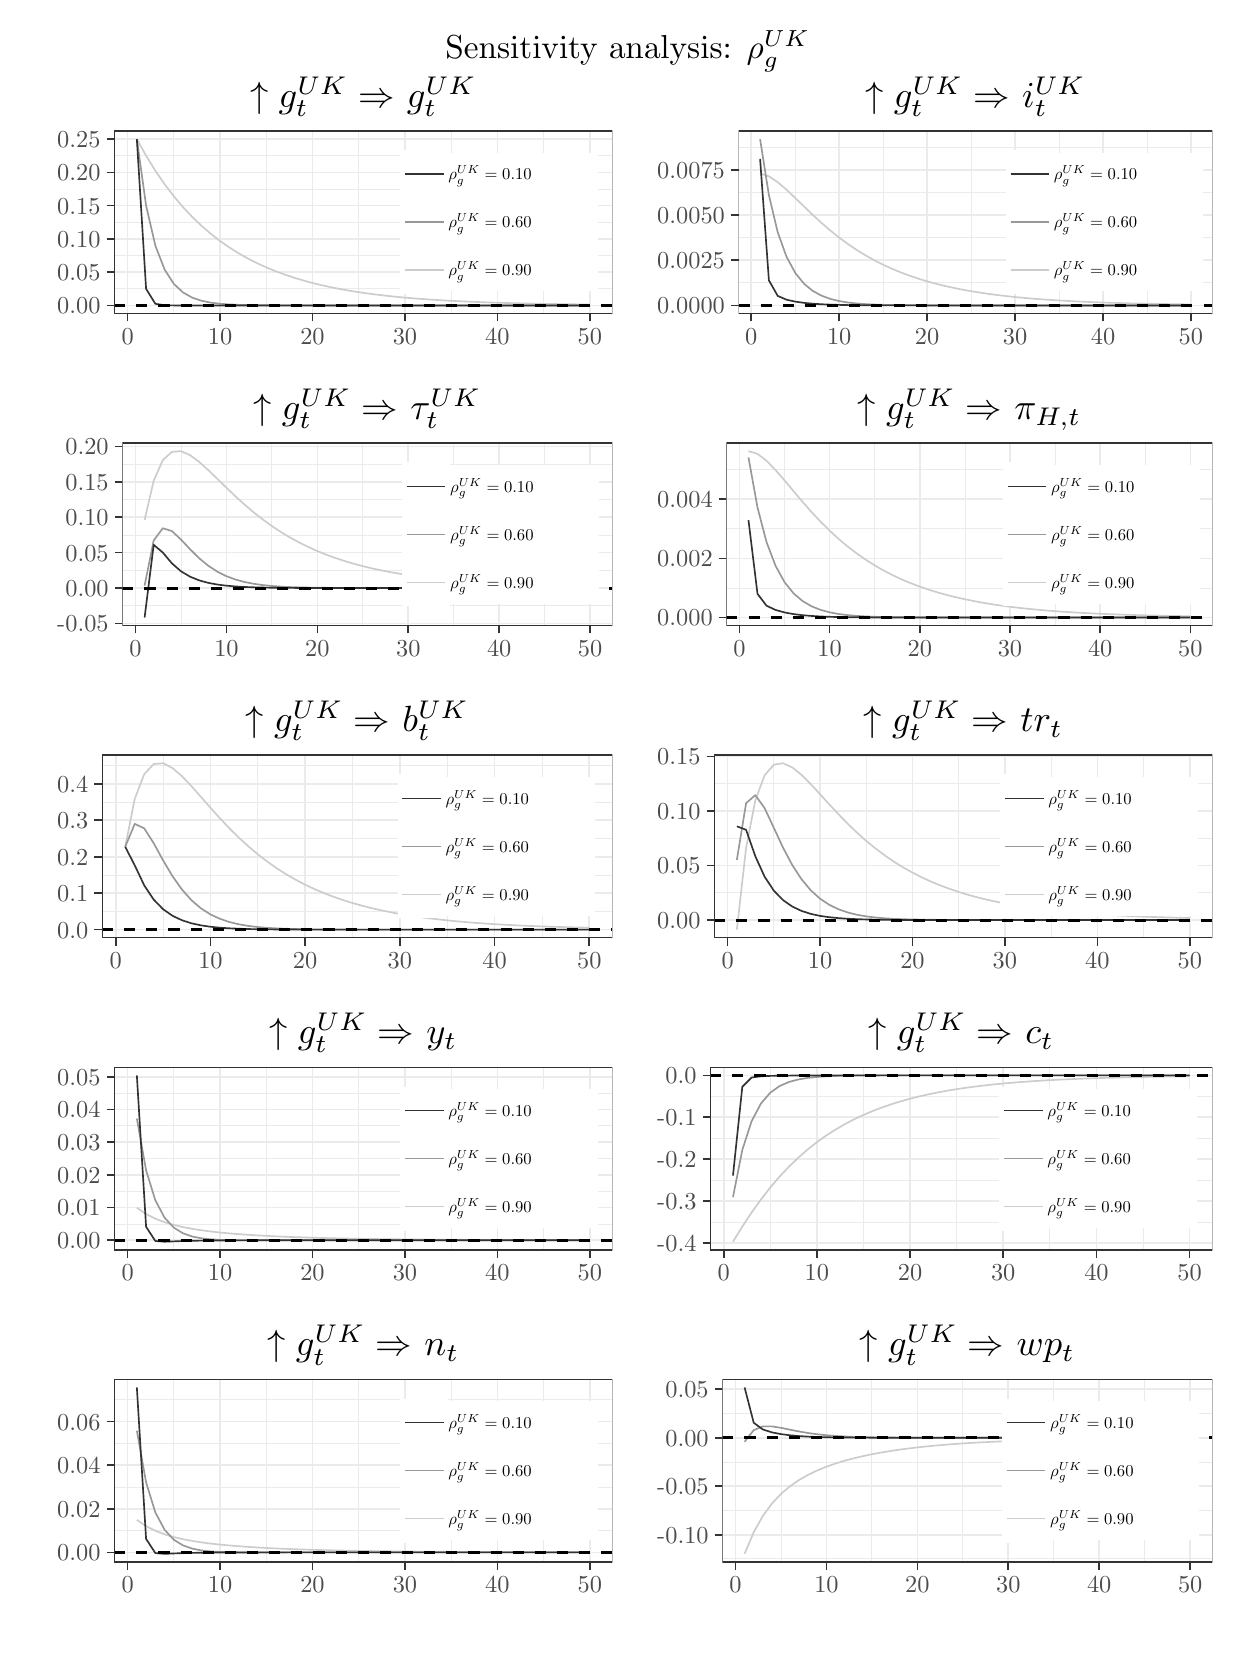
\begin{tikzpicture}[x=1pt,y=1pt]
\definecolor{fillColor}{RGB}{255,255,255}
\path[use as bounding box,fill=fillColor,fill opacity=0.00] (0,0) rectangle (433.62,578.16);
\begin{scope}
\path[clip] (  0.00,451.10) rectangle (216.81,563.87);
\definecolor{drawColor}{RGB}{255,255,255}
\definecolor{fillColor}{RGB}{255,255,255}

\path[draw=drawColor,line width= 0.6pt,line join=round,line cap=round,fill=fillColor] (  0.00,451.10) rectangle (216.81,563.87);
\end{scope}
\begin{scope}
\path[clip] ( 31.27,474.78) rectangle (211.31,540.91);
\definecolor{fillColor}{RGB}{255,255,255}

\path[fill=fillColor] ( 31.27,474.78) rectangle (211.31,540.91);
\definecolor{drawColor}{gray}{0.92}

\path[draw=drawColor,line width= 0.3pt,line join=round] ( 31.27,483.79) --
	(211.31,483.79);

\path[draw=drawColor,line width= 0.3pt,line join=round] ( 31.27,495.82) --
	(211.31,495.82);

\path[draw=drawColor,line width= 0.3pt,line join=round] ( 31.27,507.84) --
	(211.31,507.84);

\path[draw=drawColor,line width= 0.3pt,line join=round] ( 31.27,519.87) --
	(211.31,519.87);

\path[draw=drawColor,line width= 0.3pt,line join=round] ( 31.27,531.89) --
	(211.31,531.89);

\path[draw=drawColor,line width= 0.3pt,line join=round] ( 52.81,474.78) --
	( 52.81,540.91);

\path[draw=drawColor,line width= 0.3pt,line join=round] ( 86.22,474.78) --
	( 86.22,540.91);

\path[draw=drawColor,line width= 0.3pt,line join=round] (119.62,474.78) --
	(119.62,540.91);

\path[draw=drawColor,line width= 0.3pt,line join=round] (153.02,474.78) --
	(153.02,540.91);

\path[draw=drawColor,line width= 0.3pt,line join=round] (186.43,474.78) --
	(186.43,540.91);

\path[draw=drawColor,line width= 0.6pt,line join=round] ( 31.27,477.78) --
	(211.31,477.78);

\path[draw=drawColor,line width= 0.6pt,line join=round] ( 31.27,489.81) --
	(211.31,489.81);

\path[draw=drawColor,line width= 0.6pt,line join=round] ( 31.27,501.83) --
	(211.31,501.83);

\path[draw=drawColor,line width= 0.6pt,line join=round] ( 31.27,513.86) --
	(211.31,513.86);

\path[draw=drawColor,line width= 0.6pt,line join=round] ( 31.27,525.88) --
	(211.31,525.88);

\path[draw=drawColor,line width= 0.6pt,line join=round] ( 31.27,537.90) --
	(211.31,537.90);

\path[draw=drawColor,line width= 0.6pt,line join=round] ( 36.11,474.78) --
	( 36.11,540.91);

\path[draw=drawColor,line width= 0.6pt,line join=round] ( 69.52,474.78) --
	( 69.52,540.91);

\path[draw=drawColor,line width= 0.6pt,line join=round] (102.92,474.78) --
	(102.92,540.91);

\path[draw=drawColor,line width= 0.6pt,line join=round] (136.32,474.78) --
	(136.32,540.91);

\path[draw=drawColor,line width= 0.6pt,line join=round] (169.72,474.78) --
	(169.72,540.91);

\path[draw=drawColor,line width= 0.6pt,line join=round] (203.13,474.78) --
	(203.13,540.91);
\definecolor{drawColor}{gray}{0.80}

\path[draw=drawColor,line width= 0.6pt,line join=round] ( 39.45,537.90) --
	( 42.79,531.89) --
	( 46.13,526.48) --
	( 49.47,521.61) --
	( 52.81,517.23) --
	( 56.15,513.28) --
	( 59.50,509.73) --
	( 62.84,506.54) --
	( 66.18,503.66) --
	( 69.52,501.07) --
	( 72.86,498.75) --
	( 76.20,496.65) --
	( 79.54,494.76) --
	( 82.88,493.06) --
	( 86.22,491.54) --
	( 89.56,490.16) --
	( 92.90,488.92) --
	( 96.24,487.81) --
	( 99.58,486.81) --
	(102.92,485.90) --
	(106.26,485.09) --
	(109.60,484.36) --
	(112.94,483.70) --
	(116.28,483.11) --
	(119.62,482.58) --
	(122.96,482.10) --
	(126.30,481.67) --
	(129.64,481.28) --
	(132.98,480.93) --
	(136.32,480.61) --
	(139.66,480.33) --
	(143.00,480.08) --
	(146.34,479.85) --
	(149.68,479.64) --
	(153.02,479.45) --
	(156.36,479.29) --
	(159.70,479.14) --
	(163.04,479.00) --
	(166.38,478.88) --
	(169.72,478.77) --
	(173.06,478.67) --
	(176.40,478.58) --
	(179.74,478.50) --
	(183.08,478.43) --
	(186.43,478.36) --
	(189.77,478.31) --
	(193.11,478.25) --
	(196.45,478.21) --
	(199.79,478.16) --
	(203.13,478.13);
\definecolor{drawColor}{RGB}{152,152,152}

\path[draw=drawColor,line width= 0.6pt,line join=round] ( 39.45,537.90) --
	( 42.79,513.86) --
	( 46.13,499.43) --
	( 49.47,490.77) --
	( 52.81,485.57) --
	( 56.15,482.46) --
	( 59.50,480.59) --
	( 62.84,479.46) --
	( 66.18,478.79) --
	( 69.52,478.39) --
	( 72.86,478.15) --
	( 76.20,478.00) --
	( 79.54,477.91) --
	( 82.88,477.86) --
	( 86.22,477.83) --
	( 89.56,477.81) --
	( 92.90,477.80) --
	( 96.24,477.79) --
	( 99.58,477.79) --
	(102.92,477.79) --
	(106.26,477.78) --
	(109.60,477.78) --
	(112.94,477.78) --
	(116.28,477.78) --
	(119.62,477.78) --
	(122.96,477.78) --
	(126.30,477.78) --
	(129.64,477.78) --
	(132.98,477.78) --
	(136.32,477.78) --
	(139.66,477.78) --
	(143.00,477.78) --
	(146.34,477.78) --
	(149.68,477.78) --
	(153.02,477.78) --
	(156.36,477.78) --
	(159.70,477.78) --
	(163.04,477.78) --
	(166.38,477.78) --
	(169.72,477.78) --
	(173.06,477.78) --
	(176.40,477.78) --
	(179.74,477.78) --
	(183.08,477.78) --
	(186.43,477.78) --
	(189.77,477.78) --
	(193.11,477.78) --
	(196.45,477.78) --
	(199.79,477.78) --
	(203.13,477.78);
\definecolor{drawColor}{gray}{0.20}

\path[draw=drawColor,line width= 0.6pt,line join=round] ( 39.45,537.90) --
	( 42.79,483.79) --
	( 46.13,478.38) --
	( 49.47,477.84) --
	( 52.81,477.79) --
	( 56.15,477.78) --
	( 59.50,477.78) --
	( 62.84,477.78) --
	( 66.18,477.78) --
	( 69.52,477.78) --
	( 72.86,477.78) --
	( 76.20,477.78) --
	( 79.54,477.78) --
	( 82.88,477.78) --
	( 86.22,477.78) --
	( 89.56,477.78) --
	( 92.90,477.78) --
	( 96.24,477.78) --
	( 99.58,477.78) --
	(102.92,477.78) --
	(106.26,477.78) --
	(109.60,477.78) --
	(112.94,477.78) --
	(116.28,477.78) --
	(119.62,477.78) --
	(122.96,477.78) --
	(126.30,477.78) --
	(129.64,477.78) --
	(132.98,477.78) --
	(136.32,477.78) --
	(139.66,477.78) --
	(143.00,477.78) --
	(146.34,477.78) --
	(149.68,477.78) --
	(153.02,477.78) --
	(156.36,477.78) --
	(159.70,477.78) --
	(163.04,477.78) --
	(166.38,477.78) --
	(169.72,477.78) --
	(173.06,477.78) --
	(176.40,477.78) --
	(179.74,477.78) --
	(183.08,477.78) --
	(186.43,477.78) --
	(189.77,477.78) --
	(193.11,477.78) --
	(196.45,477.78) --
	(199.79,477.78) --
	(203.13,477.78);
\definecolor{drawColor}{RGB}{0,0,0}

\path[draw=drawColor,line width= 1.1pt,dash pattern=on 4pt off 4pt ,line join=round] ( 31.27,477.78) -- (211.31,477.78);
\definecolor{drawColor}{gray}{0.20}

\path[draw=drawColor,line width= 0.6pt,line join=round,line cap=round] ( 31.27,474.78) rectangle (211.31,540.91);
\end{scope}
\begin{scope}
\path[clip] (  0.00,  0.00) rectangle (433.62,578.16);
\definecolor{drawColor}{gray}{0.30}

\node[text=drawColor,anchor=base east,inner sep=0pt, outer sep=0pt, scale=  0.88] at ( 26.32,474.75) {0.00};

\node[text=drawColor,anchor=base east,inner sep=0pt, outer sep=0pt, scale=  0.88] at ( 26.32,486.78) {0.05};

\node[text=drawColor,anchor=base east,inner sep=0pt, outer sep=0pt, scale=  0.88] at ( 26.32,498.80) {0.10};

\node[text=drawColor,anchor=base east,inner sep=0pt, outer sep=0pt, scale=  0.88] at ( 26.32,510.83) {0.15};

\node[text=drawColor,anchor=base east,inner sep=0pt, outer sep=0pt, scale=  0.88] at ( 26.32,522.85) {0.20};

\node[text=drawColor,anchor=base east,inner sep=0pt, outer sep=0pt, scale=  0.88] at ( 26.32,534.87) {0.25};
\end{scope}
\begin{scope}
\path[clip] (  0.00,  0.00) rectangle (433.62,578.16);
\definecolor{drawColor}{gray}{0.20}

\path[draw=drawColor,line width= 0.6pt,line join=round] ( 28.52,477.78) --
	( 31.27,477.78);

\path[draw=drawColor,line width= 0.6pt,line join=round] ( 28.52,489.81) --
	( 31.27,489.81);

\path[draw=drawColor,line width= 0.6pt,line join=round] ( 28.52,501.83) --
	( 31.27,501.83);

\path[draw=drawColor,line width= 0.6pt,line join=round] ( 28.52,513.86) --
	( 31.27,513.86);

\path[draw=drawColor,line width= 0.6pt,line join=round] ( 28.52,525.88) --
	( 31.27,525.88);

\path[draw=drawColor,line width= 0.6pt,line join=round] ( 28.52,537.90) --
	( 31.27,537.90);
\end{scope}
\begin{scope}
\path[clip] (  0.00,  0.00) rectangle (433.62,578.16);
\definecolor{drawColor}{gray}{0.20}

\path[draw=drawColor,line width= 0.6pt,line join=round] ( 36.11,472.03) --
	( 36.11,474.78);

\path[draw=drawColor,line width= 0.6pt,line join=round] ( 69.52,472.03) --
	( 69.52,474.78);

\path[draw=drawColor,line width= 0.6pt,line join=round] (102.92,472.03) --
	(102.92,474.78);

\path[draw=drawColor,line width= 0.6pt,line join=round] (136.32,472.03) --
	(136.32,474.78);

\path[draw=drawColor,line width= 0.6pt,line join=round] (169.72,472.03) --
	(169.72,474.78);

\path[draw=drawColor,line width= 0.6pt,line join=round] (203.13,472.03) --
	(203.13,474.78);
\end{scope}
\begin{scope}
\path[clip] (  0.00,  0.00) rectangle (433.62,578.16);
\definecolor{drawColor}{gray}{0.30}

\node[text=drawColor,anchor=base,inner sep=0pt, outer sep=0pt, scale=  0.88] at ( 36.11,463.76) {0};

\node[text=drawColor,anchor=base,inner sep=0pt, outer sep=0pt, scale=  0.88] at ( 69.52,463.76) {10};

\node[text=drawColor,anchor=base,inner sep=0pt, outer sep=0pt, scale=  0.88] at (102.92,463.76) {20};

\node[text=drawColor,anchor=base,inner sep=0pt, outer sep=0pt, scale=  0.88] at (136.32,463.76) {30};

\node[text=drawColor,anchor=base,inner sep=0pt, outer sep=0pt, scale=  0.88] at (169.72,463.76) {40};

\node[text=drawColor,anchor=base,inner sep=0pt, outer sep=0pt, scale=  0.88] at (203.13,463.76) {50};
\end{scope}
\begin{scope}
\path[clip] (  0.00,  0.00) rectangle (433.62,578.16);
\definecolor{fillColor}{RGB}{255,255,255}

\path[fill=fillColor] (135.68,482.83) rectangle (205.92,532.86);
\end{scope}
\begin{scope}
\path[clip] (  0.00,  0.00) rectangle (433.62,578.16);
\definecolor{fillColor}{RGB}{255,255,255}

\path[fill=fillColor] (134.68,516.52) rectangle (152.03,533.86);
\end{scope}
\begin{scope}
\path[clip] (  0.00,  0.00) rectangle (433.62,578.16);
\definecolor{drawColor}{gray}{0.20}

\path[draw=drawColor,line width= 0.6pt,line join=round] (136.42,525.19) -- (150.29,525.19);
\end{scope}
\begin{scope}
\path[clip] (  0.00,  0.00) rectangle (433.62,578.16);
\definecolor{drawColor}{gray}{0.20}

\path[draw=drawColor,line width= 0.6pt,line join=round] (136.42,525.19) -- (150.29,525.19);
\end{scope}
\begin{scope}
\path[clip] (  0.00,  0.00) rectangle (433.62,578.16);
\definecolor{drawColor}{gray}{0.20}

\path[draw=drawColor,line width= 0.6pt,line join=round] (136.42,525.19) -- (150.29,525.19);
\end{scope}
\begin{scope}
\path[clip] (  0.00,  0.00) rectangle (433.62,578.16);
\definecolor{fillColor}{RGB}{255,255,255}

\path[fill=fillColor] (134.68,499.17) rectangle (152.03,516.52);
\end{scope}
\begin{scope}
\path[clip] (  0.00,  0.00) rectangle (433.62,578.16);
\definecolor{drawColor}{RGB}{152,152,152}

\path[draw=drawColor,line width= 0.6pt,line join=round] (136.42,507.84) -- (150.29,507.84);
\end{scope}
\begin{scope}
\path[clip] (  0.00,  0.00) rectangle (433.62,578.16);
\definecolor{drawColor}{RGB}{152,152,152}

\path[draw=drawColor,line width= 0.6pt,line join=round] (136.42,507.84) -- (150.29,507.84);
\end{scope}
\begin{scope}
\path[clip] (  0.00,  0.00) rectangle (433.62,578.16);
\definecolor{drawColor}{RGB}{152,152,152}

\path[draw=drawColor,line width= 0.6pt,line join=round] (136.42,507.84) -- (150.29,507.84);
\end{scope}
\begin{scope}
\path[clip] (  0.00,  0.00) rectangle (433.62,578.16);
\definecolor{fillColor}{RGB}{255,255,255}

\path[fill=fillColor] (134.68,481.83) rectangle (152.03,499.17);
\end{scope}
\begin{scope}
\path[clip] (  0.00,  0.00) rectangle (433.62,578.16);
\definecolor{drawColor}{gray}{0.80}

\path[draw=drawColor,line width= 0.6pt,line join=round] (136.42,490.50) -- (150.29,490.50);
\end{scope}
\begin{scope}
\path[clip] (  0.00,  0.00) rectangle (433.62,578.16);
\definecolor{drawColor}{gray}{0.80}

\path[draw=drawColor,line width= 0.6pt,line join=round] (136.42,490.50) -- (150.29,490.50);
\end{scope}
\begin{scope}
\path[clip] (  0.00,  0.00) rectangle (433.62,578.16);
\definecolor{drawColor}{gray}{0.80}

\path[draw=drawColor,line width= 0.6pt,line join=round] (136.42,490.50) -- (150.29,490.50);
\end{scope}
\begin{scope}
\path[clip] (  0.00,  0.00) rectangle (433.62,578.16);
\definecolor{drawColor}{RGB}{0,0,0}

\node[text=drawColor,anchor=base west,inner sep=0pt, outer sep=0pt, scale=  0.60] at (152.03,523.12) {${\rho_g^{UK}}=0.10$};
\end{scope}
\begin{scope}
\path[clip] (  0.00,  0.00) rectangle (433.62,578.16);
\definecolor{drawColor}{RGB}{0,0,0}

\node[text=drawColor,anchor=base west,inner sep=0pt, outer sep=0pt, scale=  0.60] at (152.03,505.78) {${\rho_g^{UK}}=0.60$};
\end{scope}
\begin{scope}
\path[clip] (  0.00,  0.00) rectangle (433.62,578.16);
\definecolor{drawColor}{RGB}{0,0,0}

\node[text=drawColor,anchor=base west,inner sep=0pt, outer sep=0pt, scale=  0.60] at (152.03,488.43) {${\rho_g^{UK}}=0.90$};
\end{scope}
\begin{scope}
\path[clip] (  0.00,  0.00) rectangle (433.62,578.16);
\definecolor{drawColor}{RGB}{0,0,0}

\node[text=drawColor,anchor=base,inner sep=0pt, outer sep=0pt, scale=  1.32] at (121.29,549.28) {$\uparrow  g^{UK}_t \Rightarrow $ ${g^{UK}_t}$};
\end{scope}
\begin{scope}
\path[clip] (216.81,451.10) rectangle (433.62,563.87);
\definecolor{drawColor}{RGB}{255,255,255}
\definecolor{fillColor}{RGB}{255,255,255}

\path[draw=drawColor,line width= 0.6pt,line join=round,line cap=round,fill=fillColor] (216.81,451.10) rectangle (433.62,563.87);
\end{scope}
\begin{scope}
\path[clip] (256.88,474.78) rectangle (428.12,540.91);
\definecolor{fillColor}{RGB}{255,255,255}

\path[fill=fillColor] (256.88,474.78) rectangle (428.12,540.91);
\definecolor{drawColor}{gray}{0.92}

\path[draw=drawColor,line width= 0.3pt,line join=round] (256.88,485.94) --
	(428.12,485.94);

\path[draw=drawColor,line width= 0.3pt,line join=round] (256.88,502.26) --
	(428.12,502.26);

\path[draw=drawColor,line width= 0.3pt,line join=round] (256.88,518.58) --
	(428.12,518.58);

\path[draw=drawColor,line width= 0.3pt,line join=round] (256.88,534.91) --
	(428.12,534.91);

\path[draw=drawColor,line width= 0.3pt,line join=round] (277.37,474.78) --
	(277.37,540.91);

\path[draw=drawColor,line width= 0.3pt,line join=round] (309.14,474.78) --
	(309.14,540.91);

\path[draw=drawColor,line width= 0.3pt,line join=round] (340.91,474.78) --
	(340.91,540.91);

\path[draw=drawColor,line width= 0.3pt,line join=round] (372.68,474.78) --
	(372.68,540.91);

\path[draw=drawColor,line width= 0.3pt,line join=round] (404.45,474.78) --
	(404.45,540.91);

\path[draw=drawColor,line width= 0.6pt,line join=round] (256.88,477.78) --
	(428.12,477.78);

\path[draw=drawColor,line width= 0.6pt,line join=round] (256.88,494.10) --
	(428.12,494.10);

\path[draw=drawColor,line width= 0.6pt,line join=round] (256.88,510.42) --
	(428.12,510.42);

\path[draw=drawColor,line width= 0.6pt,line join=round] (256.88,526.74) --
	(428.12,526.74);

\path[draw=drawColor,line width= 0.6pt,line join=round] (261.48,474.78) --
	(261.48,540.91);

\path[draw=drawColor,line width= 0.6pt,line join=round] (293.25,474.78) --
	(293.25,540.91);

\path[draw=drawColor,line width= 0.6pt,line join=round] (325.03,474.78) --
	(325.03,540.91);

\path[draw=drawColor,line width= 0.6pt,line join=round] (356.80,474.78) --
	(356.80,540.91);

\path[draw=drawColor,line width= 0.6pt,line join=round] (388.57,474.78) --
	(388.57,540.91);

\path[draw=drawColor,line width= 0.6pt,line join=round] (420.34,474.78) --
	(420.34,540.91);
\definecolor{drawColor}{gray}{0.80}

\path[draw=drawColor,line width= 0.6pt,line join=round] (264.66,525.44) --
	(267.84,524.45) --
	(271.02,522.33) --
	(274.19,519.61) --
	(277.37,516.59) --
	(280.55,513.51) --
	(283.72,510.47) --
	(286.90,507.56) --
	(290.08,504.83) --
	(293.25,502.29) --
	(296.43,499.95) --
	(299.61,497.81) --
	(302.79,495.86) --
	(305.96,494.09) --
	(309.14,492.48) --
	(312.32,491.03) --
	(315.49,489.71) --
	(318.67,488.53) --
	(321.85,487.46) --
	(325.03,486.49) --
	(328.20,485.62) --
	(331.38,484.84) --
	(334.56,484.14) --
	(337.73,483.50) --
	(340.91,482.93) --
	(344.09,482.42) --
	(347.26,481.95) --
	(350.44,481.54) --
	(353.62,481.16) --
	(356.80,480.82) --
	(359.97,480.52) --
	(363.15,480.24) --
	(366.33,480.00) --
	(369.50,479.78) --
	(372.68,479.58) --
	(375.86,479.40) --
	(379.03,479.24) --
	(382.21,479.09) --
	(385.39,478.96) --
	(388.57,478.84) --
	(391.74,478.74) --
	(394.92,478.64) --
	(398.10,478.55) --
	(401.27,478.48) --
	(404.45,478.41) --
	(407.63,478.35) --
	(410.81,478.29) --
	(413.98,478.24) --
	(417.16,478.19) --
	(420.34,478.15);
\definecolor{drawColor}{RGB}{152,152,152}

\path[draw=drawColor,line width= 0.6pt,line join=round] (264.66,537.90) --
	(267.84,517.63) --
	(271.02,504.24) --
	(274.19,495.39) --
	(277.37,489.52) --
	(280.55,485.61) --
	(283.72,483.02) --
	(286.90,481.29) --
	(290.08,480.13) --
	(293.25,479.36) --
	(296.43,478.84) --
	(299.61,478.49) --
	(302.79,478.26) --
	(305.96,478.10) --
	(309.14,478.00) --
	(312.32,477.93) --
	(315.49,477.88) --
	(318.67,477.85) --
	(321.85,477.83) --
	(325.03,477.81) --
	(328.20,477.80) --
	(331.38,477.80) --
	(334.56,477.79) --
	(337.73,477.79) --
	(340.91,477.79) --
	(344.09,477.78) --
	(347.26,477.78) --
	(350.44,477.78) --
	(353.62,477.78) --
	(356.80,477.78) --
	(359.97,477.78) --
	(363.15,477.78) --
	(366.33,477.78) --
	(369.50,477.78) --
	(372.68,477.78) --
	(375.86,477.78) --
	(379.03,477.78) --
	(382.21,477.78) --
	(385.39,477.78) --
	(388.57,477.78) --
	(391.74,477.78) --
	(394.92,477.78) --
	(398.10,477.78) --
	(401.27,477.78) --
	(404.45,477.78) --
	(407.63,477.78) --
	(410.81,477.78) --
	(413.98,477.78) --
	(417.16,477.78) --
	(420.34,477.78);
\definecolor{drawColor}{gray}{0.20}

\path[draw=drawColor,line width= 0.6pt,line join=round] (264.66,530.73) --
	(267.84,486.85) --
	(271.02,481.24) --
	(274.19,479.86) --
	(277.37,479.16) --
	(280.55,478.71) --
	(283.72,478.41) --
	(286.90,478.21) --
	(290.08,478.07) --
	(293.25,477.98) --
	(296.43,477.91) --
	(299.61,477.87) --
	(302.79,477.84) --
	(305.96,477.82) --
	(309.14,477.81) --
	(312.32,477.80) --
	(315.49,477.79) --
	(318.67,477.79) --
	(321.85,477.79) --
	(325.03,477.79) --
	(328.20,477.78) --
	(331.38,477.78) --
	(334.56,477.78) --
	(337.73,477.78) --
	(340.91,477.78) --
	(344.09,477.78) --
	(347.26,477.78) --
	(350.44,477.78) --
	(353.62,477.78) --
	(356.80,477.78) --
	(359.97,477.78) --
	(363.15,477.78) --
	(366.33,477.78) --
	(369.50,477.78) --
	(372.68,477.78) --
	(375.86,477.78) --
	(379.03,477.78) --
	(382.21,477.78) --
	(385.39,477.78) --
	(388.57,477.78) --
	(391.74,477.78) --
	(394.92,477.78) --
	(398.10,477.78) --
	(401.27,477.78) --
	(404.45,477.78) --
	(407.63,477.78) --
	(410.81,477.78) --
	(413.98,477.78) --
	(417.16,477.78) --
	(420.34,477.78);
\definecolor{drawColor}{RGB}{0,0,0}

\path[draw=drawColor,line width= 1.1pt,dash pattern=on 4pt off 4pt ,line join=round] (256.88,477.78) -- (428.12,477.78);
\definecolor{drawColor}{gray}{0.20}

\path[draw=drawColor,line width= 0.6pt,line join=round,line cap=round] (256.88,474.78) rectangle (428.12,540.91);
\end{scope}
\begin{scope}
\path[clip] (  0.00,  0.00) rectangle (433.62,578.16);
\definecolor{drawColor}{gray}{0.30}

\node[text=drawColor,anchor=base east,inner sep=0pt, outer sep=0pt, scale=  0.88] at (251.93,474.75) {0.0000};

\node[text=drawColor,anchor=base east,inner sep=0pt, outer sep=0pt, scale=  0.88] at (251.93,491.07) {0.0025};

\node[text=drawColor,anchor=base east,inner sep=0pt, outer sep=0pt, scale=  0.88] at (251.93,507.39) {0.0050};

\node[text=drawColor,anchor=base east,inner sep=0pt, outer sep=0pt, scale=  0.88] at (251.93,523.71) {0.0075};
\end{scope}
\begin{scope}
\path[clip] (  0.00,  0.00) rectangle (433.62,578.16);
\definecolor{drawColor}{gray}{0.20}

\path[draw=drawColor,line width= 0.6pt,line join=round] (254.13,477.78) --
	(256.88,477.78);

\path[draw=drawColor,line width= 0.6pt,line join=round] (254.13,494.10) --
	(256.88,494.10);

\path[draw=drawColor,line width= 0.6pt,line join=round] (254.13,510.42) --
	(256.88,510.42);

\path[draw=drawColor,line width= 0.6pt,line join=round] (254.13,526.74) --
	(256.88,526.74);
\end{scope}
\begin{scope}
\path[clip] (  0.00,  0.00) rectangle (433.62,578.16);
\definecolor{drawColor}{gray}{0.20}

\path[draw=drawColor,line width= 0.6pt,line join=round] (261.48,472.03) --
	(261.48,474.78);

\path[draw=drawColor,line width= 0.6pt,line join=round] (293.25,472.03) --
	(293.25,474.78);

\path[draw=drawColor,line width= 0.6pt,line join=round] (325.03,472.03) --
	(325.03,474.78);

\path[draw=drawColor,line width= 0.6pt,line join=round] (356.80,472.03) --
	(356.80,474.78);

\path[draw=drawColor,line width= 0.6pt,line join=round] (388.57,472.03) --
	(388.57,474.78);

\path[draw=drawColor,line width= 0.6pt,line join=round] (420.34,472.03) --
	(420.34,474.78);
\end{scope}
\begin{scope}
\path[clip] (  0.00,  0.00) rectangle (433.62,578.16);
\definecolor{drawColor}{gray}{0.30}

\node[text=drawColor,anchor=base,inner sep=0pt, outer sep=0pt, scale=  0.88] at (261.48,463.76) {0};

\node[text=drawColor,anchor=base,inner sep=0pt, outer sep=0pt, scale=  0.88] at (293.25,463.76) {10};

\node[text=drawColor,anchor=base,inner sep=0pt, outer sep=0pt, scale=  0.88] at (325.03,463.76) {20};

\node[text=drawColor,anchor=base,inner sep=0pt, outer sep=0pt, scale=  0.88] at (356.80,463.76) {30};

\node[text=drawColor,anchor=base,inner sep=0pt, outer sep=0pt, scale=  0.88] at (388.57,463.76) {40};

\node[text=drawColor,anchor=base,inner sep=0pt, outer sep=0pt, scale=  0.88] at (420.34,463.76) {50};
\end{scope}
\begin{scope}
\path[clip] (  0.00,  0.00) rectangle (433.62,578.16);
\definecolor{fillColor}{RGB}{255,255,255}

\path[fill=fillColor] (354.47,482.83) rectangle (424.71,532.86);
\end{scope}
\begin{scope}
\path[clip] (  0.00,  0.00) rectangle (433.62,578.16);
\definecolor{fillColor}{RGB}{255,255,255}

\path[fill=fillColor] (353.47,516.52) rectangle (370.82,533.86);
\end{scope}
\begin{scope}
\path[clip] (  0.00,  0.00) rectangle (433.62,578.16);
\definecolor{drawColor}{gray}{0.20}

\path[draw=drawColor,line width= 0.6pt,line join=round] (355.21,525.19) -- (369.08,525.19);
\end{scope}
\begin{scope}
\path[clip] (  0.00,  0.00) rectangle (433.62,578.16);
\definecolor{drawColor}{gray}{0.20}

\path[draw=drawColor,line width= 0.6pt,line join=round] (355.21,525.19) -- (369.08,525.19);
\end{scope}
\begin{scope}
\path[clip] (  0.00,  0.00) rectangle (433.62,578.16);
\definecolor{drawColor}{gray}{0.20}

\path[draw=drawColor,line width= 0.6pt,line join=round] (355.21,525.19) -- (369.08,525.19);
\end{scope}
\begin{scope}
\path[clip] (  0.00,  0.00) rectangle (433.62,578.16);
\definecolor{fillColor}{RGB}{255,255,255}

\path[fill=fillColor] (353.47,499.17) rectangle (370.82,516.52);
\end{scope}
\begin{scope}
\path[clip] (  0.00,  0.00) rectangle (433.62,578.16);
\definecolor{drawColor}{RGB}{152,152,152}

\path[draw=drawColor,line width= 0.6pt,line join=round] (355.21,507.84) -- (369.08,507.84);
\end{scope}
\begin{scope}
\path[clip] (  0.00,  0.00) rectangle (433.62,578.16);
\definecolor{drawColor}{RGB}{152,152,152}

\path[draw=drawColor,line width= 0.6pt,line join=round] (355.21,507.84) -- (369.08,507.84);
\end{scope}
\begin{scope}
\path[clip] (  0.00,  0.00) rectangle (433.62,578.16);
\definecolor{drawColor}{RGB}{152,152,152}

\path[draw=drawColor,line width= 0.6pt,line join=round] (355.21,507.84) -- (369.08,507.84);
\end{scope}
\begin{scope}
\path[clip] (  0.00,  0.00) rectangle (433.62,578.16);
\definecolor{fillColor}{RGB}{255,255,255}

\path[fill=fillColor] (353.47,481.83) rectangle (370.82,499.17);
\end{scope}
\begin{scope}
\path[clip] (  0.00,  0.00) rectangle (433.62,578.16);
\definecolor{drawColor}{gray}{0.80}

\path[draw=drawColor,line width= 0.6pt,line join=round] (355.21,490.50) -- (369.08,490.50);
\end{scope}
\begin{scope}
\path[clip] (  0.00,  0.00) rectangle (433.62,578.16);
\definecolor{drawColor}{gray}{0.80}

\path[draw=drawColor,line width= 0.6pt,line join=round] (355.21,490.50) -- (369.08,490.50);
\end{scope}
\begin{scope}
\path[clip] (  0.00,  0.00) rectangle (433.62,578.16);
\definecolor{drawColor}{gray}{0.80}

\path[draw=drawColor,line width= 0.6pt,line join=round] (355.21,490.50) -- (369.08,490.50);
\end{scope}
\begin{scope}
\path[clip] (  0.00,  0.00) rectangle (433.62,578.16);
\definecolor{drawColor}{RGB}{0,0,0}

\node[text=drawColor,anchor=base west,inner sep=0pt, outer sep=0pt, scale=  0.60] at (370.82,523.12) {${\rho_g^{UK}}=0.10$};
\end{scope}
\begin{scope}
\path[clip] (  0.00,  0.00) rectangle (433.62,578.16);
\definecolor{drawColor}{RGB}{0,0,0}

\node[text=drawColor,anchor=base west,inner sep=0pt, outer sep=0pt, scale=  0.60] at (370.82,505.78) {${\rho_g^{UK}}=0.60$};
\end{scope}
\begin{scope}
\path[clip] (  0.00,  0.00) rectangle (433.62,578.16);
\definecolor{drawColor}{RGB}{0,0,0}

\node[text=drawColor,anchor=base west,inner sep=0pt, outer sep=0pt, scale=  0.60] at (370.82,488.43) {${\rho_g^{UK}}=0.90$};
\end{scope}
\begin{scope}
\path[clip] (  0.00,  0.00) rectangle (433.62,578.16);
\definecolor{drawColor}{RGB}{0,0,0}

\node[text=drawColor,anchor=base,inner sep=0pt, outer sep=0pt, scale=  1.32] at (342.50,549.28) {$\uparrow  g^{UK}_t \Rightarrow $ ${i^{UK}_t}$};
\end{scope}
\begin{scope}
\path[clip] (  0.00,338.32) rectangle (216.81,451.10);
\definecolor{drawColor}{RGB}{255,255,255}
\definecolor{fillColor}{RGB}{255,255,255}

\path[draw=drawColor,line width= 0.6pt,line join=round,line cap=round,fill=fillColor] (  0.00,338.32) rectangle (216.81,451.10);
\end{scope}
\begin{scope}
\path[clip] ( 34.20,362.00) rectangle (211.31,428.14);
\definecolor{fillColor}{RGB}{255,255,255}

\path[fill=fillColor] ( 34.20,362.00) rectangle (211.31,428.14);
\definecolor{drawColor}{gray}{0.92}

\path[draw=drawColor,line width= 0.3pt,line join=round] ( 34.20,369.27) --
	(211.31,369.27);

\path[draw=drawColor,line width= 0.3pt,line join=round] ( 34.20,382.06) --
	(211.31,382.06);

\path[draw=drawColor,line width= 0.3pt,line join=round] ( 34.20,394.85) --
	(211.31,394.85);

\path[draw=drawColor,line width= 0.3pt,line join=round] ( 34.20,407.64) --
	(211.31,407.64);

\path[draw=drawColor,line width= 0.3pt,line join=round] ( 34.20,420.43) --
	(211.31,420.43);

\path[draw=drawColor,line width= 0.3pt,line join=round] ( 55.40,362.00) --
	( 55.40,428.14);

\path[draw=drawColor,line width= 0.3pt,line join=round] ( 88.25,362.00) --
	( 88.25,428.14);

\path[draw=drawColor,line width= 0.3pt,line join=round] (121.11,362.00) --
	(121.11,428.14);

\path[draw=drawColor,line width= 0.3pt,line join=round] (153.97,362.00) --
	(153.97,428.14);

\path[draw=drawColor,line width= 0.3pt,line join=round] (186.83,362.00) --
	(186.83,428.14);

\path[draw=drawColor,line width= 0.6pt,line join=round] ( 34.20,362.87) --
	(211.31,362.87);

\path[draw=drawColor,line width= 0.6pt,line join=round] ( 34.20,375.66) --
	(211.31,375.66);

\path[draw=drawColor,line width= 0.6pt,line join=round] ( 34.20,388.45) --
	(211.31,388.45);

\path[draw=drawColor,line width= 0.6pt,line join=round] ( 34.20,401.24) --
	(211.31,401.24);

\path[draw=drawColor,line width= 0.6pt,line join=round] ( 34.20,414.03) --
	(211.31,414.03);

\path[draw=drawColor,line width= 0.6pt,line join=round] ( 34.20,426.82) --
	(211.31,426.82);

\path[draw=drawColor,line width= 0.6pt,line join=round] ( 38.97,362.00) --
	( 38.97,428.14);

\path[draw=drawColor,line width= 0.6pt,line join=round] ( 71.83,362.00) --
	( 71.83,428.14);

\path[draw=drawColor,line width= 0.6pt,line join=round] (104.68,362.00) --
	(104.68,428.14);

\path[draw=drawColor,line width= 0.6pt,line join=round] (137.54,362.00) --
	(137.54,428.14);

\path[draw=drawColor,line width= 0.6pt,line join=round] (170.40,362.00) --
	(170.40,428.14);

\path[draw=drawColor,line width= 0.6pt,line join=round] (203.26,362.00) --
	(203.26,428.14);
\definecolor{drawColor}{gray}{0.80}

\path[draw=drawColor,line width= 0.6pt,line join=round] ( 42.25,400.23) --
	( 45.54,414.45) --
	( 48.82,421.86) --
	( 52.11,424.88) --
	( 55.40,425.13) --
	( 58.68,423.68) --
	( 61.97,421.25) --
	( 65.25,418.29) --
	( 68.54,415.11) --
	( 71.83,411.90) --
	( 75.11,408.77) --
	( 78.40,405.80) --
	( 81.68,403.01) --
	( 84.97,400.43) --
	( 88.25,398.06) --
	( 91.54,395.89) --
	( 94.83,393.91) --
	( 98.11,392.12) --
	(101.40,390.50) --
	(104.68,389.03) --
	(107.97,387.70) --
	(111.26,386.50) --
	(114.54,385.42) --
	(117.83,384.45) --
	(121.11,383.57) --
	(124.40,382.78) --
	(127.68,382.07) --
	(130.97,381.43) --
	(134.26,380.86) --
	(137.54,380.34) --
	(140.83,379.87) --
	(144.11,379.45) --
	(147.40,379.07) --
	(150.69,378.73) --
	(153.97,378.42) --
	(157.26,378.15) --
	(160.54,377.90) --
	(163.83,377.67) --
	(167.12,377.47) --
	(170.40,377.29) --
	(173.69,377.13) --
	(176.97,376.98) --
	(180.26,376.85) --
	(183.54,376.73) --
	(186.83,376.62) --
	(190.12,376.53) --
	(193.40,376.44) --
	(196.69,376.36) --
	(199.97,376.29) --
	(203.26,376.23);
\definecolor{drawColor}{RGB}{152,152,152}

\path[draw=drawColor,line width= 0.6pt,line join=round] ( 42.25,376.53) --
	( 45.54,392.86) --
	( 48.82,397.27) --
	( 52.11,396.27) --
	( 55.40,393.19) --
	( 58.68,389.68) --
	( 61.97,386.44) --
	( 65.25,383.73) --
	( 68.54,381.59) --
	( 71.83,379.95) --
	( 75.11,378.73) --
	( 78.40,377.84) --
	( 81.68,377.20) --
	( 84.97,376.74) --
	( 88.25,376.41) --
	( 91.54,376.18) --
	( 94.83,376.02) --
	( 98.11,375.91) --
	(101.40,375.83) --
	(104.68,375.78) --
	(107.97,375.74) --
	(111.26,375.72) --
	(114.54,375.70) --
	(117.83,375.69) --
	(121.11,375.68) --
	(124.40,375.67) --
	(127.68,375.67) --
	(130.97,375.67) --
	(134.26,375.66) --
	(137.54,375.66) --
	(140.83,375.66) --
	(144.11,375.66) --
	(147.40,375.66) --
	(150.69,375.66) --
	(153.97,375.66) --
	(157.26,375.66) --
	(160.54,375.66) --
	(163.83,375.66) --
	(167.12,375.66) --
	(170.40,375.66) --
	(173.69,375.66) --
	(176.97,375.66) --
	(180.26,375.66) --
	(183.54,375.66) --
	(186.83,375.66) --
	(190.12,375.66) --
	(193.40,375.66) --
	(196.69,375.66) --
	(199.97,375.66) --
	(203.26,375.66);
\definecolor{drawColor}{gray}{0.20}

\path[draw=drawColor,line width= 0.6pt,line join=round] ( 42.25,365.01) --
	( 45.54,391.28) --
	( 48.82,388.51) --
	( 52.11,384.59) --
	( 55.40,381.72) --
	( 58.68,379.77) --
	( 61.97,378.44) --
	( 65.25,377.54) --
	( 68.54,376.93) --
	( 71.83,376.52) --
	( 75.11,376.24) --
	( 78.40,376.05) --
	( 81.68,375.93) --
	( 84.97,375.84) --
	( 88.25,375.78) --
	( 91.54,375.74) --
	( 94.83,375.72) --
	( 98.11,375.70) --
	(101.40,375.69) --
	(104.68,375.68) --
	(107.97,375.67) --
	(111.26,375.67) --
	(114.54,375.67) --
	(117.83,375.66) --
	(121.11,375.66) --
	(124.40,375.66) --
	(127.68,375.66) --
	(130.97,375.66) --
	(134.26,375.66) --
	(137.54,375.66) --
	(140.83,375.66) --
	(144.11,375.66) --
	(147.40,375.66) --
	(150.69,375.66) --
	(153.97,375.66) --
	(157.26,375.66) --
	(160.54,375.66) --
	(163.83,375.66) --
	(167.12,375.66) --
	(170.40,375.66) --
	(173.69,375.66) --
	(176.97,375.66) --
	(180.26,375.66) --
	(183.54,375.66) --
	(186.83,375.66) --
	(190.12,375.66) --
	(193.40,375.66) --
	(196.69,375.66) --
	(199.97,375.66) --
	(203.26,375.66);
\definecolor{drawColor}{RGB}{0,0,0}

\path[draw=drawColor,line width= 1.1pt,dash pattern=on 4pt off 4pt ,line join=round] ( 34.20,375.66) -- (211.31,375.66);
\definecolor{drawColor}{gray}{0.20}

\path[draw=drawColor,line width= 0.6pt,line join=round,line cap=round] ( 34.20,362.00) rectangle (211.31,428.14);
\end{scope}
\begin{scope}
\path[clip] (  0.00,  0.00) rectangle (433.62,578.16);
\definecolor{drawColor}{gray}{0.30}

\node[text=drawColor,anchor=base east,inner sep=0pt, outer sep=0pt, scale=  0.88] at ( 29.25,359.84) {-0.05};

\node[text=drawColor,anchor=base east,inner sep=0pt, outer sep=0pt, scale=  0.88] at ( 29.25,372.63) {0.00};

\node[text=drawColor,anchor=base east,inner sep=0pt, outer sep=0pt, scale=  0.88] at ( 29.25,385.42) {0.05};

\node[text=drawColor,anchor=base east,inner sep=0pt, outer sep=0pt, scale=  0.88] at ( 29.25,398.21) {0.10};

\node[text=drawColor,anchor=base east,inner sep=0pt, outer sep=0pt, scale=  0.88] at ( 29.25,411.00) {0.15};

\node[text=drawColor,anchor=base east,inner sep=0pt, outer sep=0pt, scale=  0.88] at ( 29.25,423.79) {0.20};
\end{scope}
\begin{scope}
\path[clip] (  0.00,  0.00) rectangle (433.62,578.16);
\definecolor{drawColor}{gray}{0.20}

\path[draw=drawColor,line width= 0.6pt,line join=round] ( 31.45,362.87) --
	( 34.20,362.87);

\path[draw=drawColor,line width= 0.6pt,line join=round] ( 31.45,375.66) --
	( 34.20,375.66);

\path[draw=drawColor,line width= 0.6pt,line join=round] ( 31.45,388.45) --
	( 34.20,388.45);

\path[draw=drawColor,line width= 0.6pt,line join=round] ( 31.45,401.24) --
	( 34.20,401.24);

\path[draw=drawColor,line width= 0.6pt,line join=round] ( 31.45,414.03) --
	( 34.20,414.03);

\path[draw=drawColor,line width= 0.6pt,line join=round] ( 31.45,426.82) --
	( 34.20,426.82);
\end{scope}
\begin{scope}
\path[clip] (  0.00,  0.00) rectangle (433.62,578.16);
\definecolor{drawColor}{gray}{0.20}

\path[draw=drawColor,line width= 0.6pt,line join=round] ( 38.97,359.25) --
	( 38.97,362.00);

\path[draw=drawColor,line width= 0.6pt,line join=round] ( 71.83,359.25) --
	( 71.83,362.00);

\path[draw=drawColor,line width= 0.6pt,line join=round] (104.68,359.25) --
	(104.68,362.00);

\path[draw=drawColor,line width= 0.6pt,line join=round] (137.54,359.25) --
	(137.54,362.00);

\path[draw=drawColor,line width= 0.6pt,line join=round] (170.40,359.25) --
	(170.40,362.00);

\path[draw=drawColor,line width= 0.6pt,line join=round] (203.26,359.25) --
	(203.26,362.00);
\end{scope}
\begin{scope}
\path[clip] (  0.00,  0.00) rectangle (433.62,578.16);
\definecolor{drawColor}{gray}{0.30}

\node[text=drawColor,anchor=base,inner sep=0pt, outer sep=0pt, scale=  0.88] at ( 38.97,350.99) {0};

\node[text=drawColor,anchor=base,inner sep=0pt, outer sep=0pt, scale=  0.88] at ( 71.83,350.99) {10};

\node[text=drawColor,anchor=base,inner sep=0pt, outer sep=0pt, scale=  0.88] at (104.68,350.99) {20};

\node[text=drawColor,anchor=base,inner sep=0pt, outer sep=0pt, scale=  0.88] at (137.54,350.99) {30};

\node[text=drawColor,anchor=base,inner sep=0pt, outer sep=0pt, scale=  0.88] at (170.40,350.99) {40};

\node[text=drawColor,anchor=base,inner sep=0pt, outer sep=0pt, scale=  0.88] at (203.26,350.99) {50};
\end{scope}
\begin{scope}
\path[clip] (  0.00,  0.00) rectangle (433.62,578.16);
\definecolor{fillColor}{RGB}{255,255,255}

\path[fill=fillColor] (136.34,370.05) rectangle (206.58,420.09);
\end{scope}
\begin{scope}
\path[clip] (  0.00,  0.00) rectangle (433.62,578.16);
\definecolor{fillColor}{RGB}{255,255,255}

\path[fill=fillColor] (135.34,403.74) rectangle (152.69,421.09);
\end{scope}
\begin{scope}
\path[clip] (  0.00,  0.00) rectangle (433.62,578.16);
\definecolor{drawColor}{gray}{0.20}

\path[draw=drawColor,line width= 0.6pt,line join=round] (137.08,412.41) -- (150.95,412.41);
\end{scope}
\begin{scope}
\path[clip] (  0.00,  0.00) rectangle (433.62,578.16);
\definecolor{drawColor}{gray}{0.20}

\path[draw=drawColor,line width= 0.6pt,line join=round] (137.08,412.41) -- (150.95,412.41);
\end{scope}
\begin{scope}
\path[clip] (  0.00,  0.00) rectangle (433.62,578.16);
\definecolor{drawColor}{gray}{0.20}

\path[draw=drawColor,line width= 0.6pt,line join=round] (137.08,412.41) -- (150.95,412.41);
\end{scope}
\begin{scope}
\path[clip] (  0.00,  0.00) rectangle (433.62,578.16);
\definecolor{fillColor}{RGB}{255,255,255}

\path[fill=fillColor] (135.34,386.40) rectangle (152.69,403.74);
\end{scope}
\begin{scope}
\path[clip] (  0.00,  0.00) rectangle (433.62,578.16);
\definecolor{drawColor}{RGB}{152,152,152}

\path[draw=drawColor,line width= 0.6pt,line join=round] (137.08,395.07) -- (150.95,395.07);
\end{scope}
\begin{scope}
\path[clip] (  0.00,  0.00) rectangle (433.62,578.16);
\definecolor{drawColor}{RGB}{152,152,152}

\path[draw=drawColor,line width= 0.6pt,line join=round] (137.08,395.07) -- (150.95,395.07);
\end{scope}
\begin{scope}
\path[clip] (  0.00,  0.00) rectangle (433.62,578.16);
\definecolor{drawColor}{RGB}{152,152,152}

\path[draw=drawColor,line width= 0.6pt,line join=round] (137.08,395.07) -- (150.95,395.07);
\end{scope}
\begin{scope}
\path[clip] (  0.00,  0.00) rectangle (433.62,578.16);
\definecolor{fillColor}{RGB}{255,255,255}

\path[fill=fillColor] (135.34,369.05) rectangle (152.69,386.40);
\end{scope}
\begin{scope}
\path[clip] (  0.00,  0.00) rectangle (433.62,578.16);
\definecolor{drawColor}{gray}{0.80}

\path[draw=drawColor,line width= 0.6pt,line join=round] (137.08,377.72) -- (150.95,377.72);
\end{scope}
\begin{scope}
\path[clip] (  0.00,  0.00) rectangle (433.62,578.16);
\definecolor{drawColor}{gray}{0.80}

\path[draw=drawColor,line width= 0.6pt,line join=round] (137.08,377.72) -- (150.95,377.72);
\end{scope}
\begin{scope}
\path[clip] (  0.00,  0.00) rectangle (433.62,578.16);
\definecolor{drawColor}{gray}{0.80}

\path[draw=drawColor,line width= 0.6pt,line join=round] (137.08,377.72) -- (150.95,377.72);
\end{scope}
\begin{scope}
\path[clip] (  0.00,  0.00) rectangle (433.62,578.16);
\definecolor{drawColor}{RGB}{0,0,0}

\node[text=drawColor,anchor=base west,inner sep=0pt, outer sep=0pt, scale=  0.60] at (152.69,410.35) {${\rho_g^{UK}}=0.10$};
\end{scope}
\begin{scope}
\path[clip] (  0.00,  0.00) rectangle (433.62,578.16);
\definecolor{drawColor}{RGB}{0,0,0}

\node[text=drawColor,anchor=base west,inner sep=0pt, outer sep=0pt, scale=  0.60] at (152.69,393.00) {${\rho_g^{UK}}=0.60$};
\end{scope}
\begin{scope}
\path[clip] (  0.00,  0.00) rectangle (433.62,578.16);
\definecolor{drawColor}{RGB}{0,0,0}

\node[text=drawColor,anchor=base west,inner sep=0pt, outer sep=0pt, scale=  0.60] at (152.69,375.66) {${\rho_g^{UK}}=0.90$};
\end{scope}
\begin{scope}
\path[clip] (  0.00,  0.00) rectangle (433.62,578.16);
\definecolor{drawColor}{RGB}{0,0,0}

\node[text=drawColor,anchor=base,inner sep=0pt, outer sep=0pt, scale=  1.32] at (122.76,436.51) {$\uparrow  g^{UK}_t \Rightarrow $ ${\tau^{UK}_t}$};
\end{scope}
\begin{scope}
\path[clip] (216.81,338.32) rectangle (433.62,451.10);
\definecolor{drawColor}{RGB}{255,255,255}
\definecolor{fillColor}{RGB}{255,255,255}

\path[draw=drawColor,line width= 0.6pt,line join=round,line cap=round,fill=fillColor] (216.81,338.32) rectangle (433.62,451.10);
\end{scope}
\begin{scope}
\path[clip] (252.48,362.00) rectangle (428.12,428.14);
\definecolor{fillColor}{RGB}{255,255,255}

\path[fill=fillColor] (252.48,362.00) rectangle (428.12,428.14);
\definecolor{drawColor}{gray}{0.92}

\path[draw=drawColor,line width= 0.3pt,line join=round] (252.48,375.70) --
	(428.12,375.70);

\path[draw=drawColor,line width= 0.3pt,line join=round] (252.48,397.09) --
	(428.12,397.09);

\path[draw=drawColor,line width= 0.3pt,line join=round] (252.48,418.49) --
	(428.12,418.49);

\path[draw=drawColor,line width= 0.3pt,line join=round] (273.50,362.00) --
	(273.50,428.14);

\path[draw=drawColor,line width= 0.3pt,line join=round] (306.08,362.00) --
	(306.08,428.14);

\path[draw=drawColor,line width= 0.3pt,line join=round] (338.67,362.00) --
	(338.67,428.14);

\path[draw=drawColor,line width= 0.3pt,line join=round] (371.26,362.00) --
	(371.26,428.14);

\path[draw=drawColor,line width= 0.3pt,line join=round] (403.84,362.00) --
	(403.84,428.14);

\path[draw=drawColor,line width= 0.6pt,line join=round] (252.48,365.01) --
	(428.12,365.01);

\path[draw=drawColor,line width= 0.6pt,line join=round] (252.48,386.40) --
	(428.12,386.40);

\path[draw=drawColor,line width= 0.6pt,line join=round] (252.48,407.79) --
	(428.12,407.79);

\path[draw=drawColor,line width= 0.6pt,line join=round] (257.20,362.00) --
	(257.20,428.14);

\path[draw=drawColor,line width= 0.6pt,line join=round] (289.79,362.00) --
	(289.79,428.14);

\path[draw=drawColor,line width= 0.6pt,line join=round] (322.38,362.00) --
	(322.38,428.14);

\path[draw=drawColor,line width= 0.6pt,line join=round] (354.96,362.00) --
	(354.96,428.14);

\path[draw=drawColor,line width= 0.6pt,line join=round] (387.55,362.00) --
	(387.55,428.14);

\path[draw=drawColor,line width= 0.6pt,line join=round] (420.14,362.00) --
	(420.14,428.14);
\definecolor{drawColor}{gray}{0.80}

\path[draw=drawColor,line width= 0.6pt,line join=round] (260.46,425.13) --
	(263.72,424.17) --
	(266.98,421.67) --
	(270.24,418.31) --
	(273.50,414.55) --
	(276.76,410.65) --
	(280.01,406.81) --
	(283.27,403.11) --
	(286.53,399.63) --
	(289.79,396.39) --
	(293.05,393.40) --
	(296.31,390.66) --
	(299.57,388.17) --
	(302.82,385.90) --
	(306.08,383.84) --
	(309.34,381.98) --
	(312.60,380.30) --
	(315.86,378.78) --
	(319.12,377.41) --
	(322.38,376.17) --
	(325.64,375.06) --
	(328.89,374.05) --
	(332.15,373.15) --
	(335.41,372.34) --
	(338.67,371.61) --
	(341.93,370.95) --
	(345.19,370.35) --
	(348.45,369.82) --
	(351.70,369.34) --
	(354.96,368.90) --
	(358.22,368.51) --
	(361.48,368.16) --
	(364.74,367.85) --
	(368.00,367.56) --
	(371.26,367.31) --
	(374.52,367.08) --
	(377.77,366.87) --
	(381.03,366.68) --
	(384.29,366.52) --
	(387.55,366.37) --
	(390.81,366.23) --
	(394.07,366.11) --
	(397.33,366.00) --
	(400.58,365.90) --
	(403.84,365.81) --
	(407.10,365.73) --
	(410.36,365.66) --
	(413.62,365.59) --
	(416.88,365.53) --
	(420.14,365.48);
\definecolor{drawColor}{RGB}{152,152,152}

\path[draw=drawColor,line width= 0.6pt,line join=round] (260.46,422.87) --
	(263.72,404.78) --
	(266.98,392.28) --
	(270.24,383.69) --
	(273.50,377.78) --
	(276.76,373.73) --
	(280.01,370.96) --
	(283.27,369.06) --
	(286.53,367.77) --
	(289.79,366.89) --
	(293.05,366.28) --
	(296.31,365.88) --
	(299.57,365.60) --
	(302.82,365.41) --
	(306.08,365.28) --
	(309.34,365.19) --
	(312.60,365.13) --
	(315.86,365.09) --
	(319.12,365.06) --
	(322.38,365.05) --
	(325.64,365.03) --
	(328.89,365.03) --
	(332.15,365.02) --
	(335.41,365.02) --
	(338.67,365.01) --
	(341.93,365.01) --
	(345.19,365.01) --
	(348.45,365.01) --
	(351.70,365.01) --
	(354.96,365.01) --
	(358.22,365.01) --
	(361.48,365.01) --
	(364.74,365.01) --
	(368.00,365.01) --
	(371.26,365.01) --
	(374.52,365.01) --
	(377.77,365.01) --
	(381.03,365.01) --
	(384.29,365.01) --
	(387.55,365.01) --
	(390.81,365.01) --
	(394.07,365.01) --
	(397.33,365.01) --
	(400.58,365.01) --
	(403.84,365.01) --
	(407.10,365.01) --
	(410.36,365.01) --
	(413.62,365.01) --
	(416.88,365.01) --
	(420.14,365.01);
\definecolor{drawColor}{gray}{0.20}

\path[draw=drawColor,line width= 0.6pt,line join=round] (260.46,400.19) --
	(263.72,373.57) --
	(266.98,369.28) --
	(270.24,367.75) --
	(273.50,366.85) --
	(276.76,366.25) --
	(280.01,365.85) --
	(283.27,365.58) --
	(286.53,365.39) --
	(289.79,365.27) --
	(293.05,365.18) --
	(296.31,365.13) --
	(299.57,365.09) --
	(302.82,365.06) --
	(306.08,365.04) --
	(309.34,365.03) --
	(312.60,365.02) --
	(315.86,365.02) --
	(319.12,365.01) --
	(322.38,365.01) --
	(325.64,365.01) --
	(328.89,365.01) --
	(332.15,365.01) --
	(335.41,365.01) --
	(338.67,365.01) --
	(341.93,365.01) --
	(345.19,365.01) --
	(348.45,365.01) --
	(351.70,365.01) --
	(354.96,365.01) --
	(358.22,365.01) --
	(361.48,365.01) --
	(364.74,365.01) --
	(368.00,365.01) --
	(371.26,365.01) --
	(374.52,365.01) --
	(377.77,365.01) --
	(381.03,365.01) --
	(384.29,365.01) --
	(387.55,365.01) --
	(390.81,365.01) --
	(394.07,365.01) --
	(397.33,365.01) --
	(400.58,365.01) --
	(403.84,365.01) --
	(407.10,365.01) --
	(410.36,365.01) --
	(413.62,365.01) --
	(416.88,365.01) --
	(420.14,365.01);
\definecolor{drawColor}{RGB}{0,0,0}

\path[draw=drawColor,line width= 1.1pt,dash pattern=on 4pt off 4pt ,line join=round] (252.48,365.01) -- (428.12,365.01);
\definecolor{drawColor}{gray}{0.20}

\path[draw=drawColor,line width= 0.6pt,line join=round,line cap=round] (252.48,362.00) rectangle (428.12,428.14);
\end{scope}
\begin{scope}
\path[clip] (  0.00,  0.00) rectangle (433.62,578.16);
\definecolor{drawColor}{gray}{0.30}

\node[text=drawColor,anchor=base east,inner sep=0pt, outer sep=0pt, scale=  0.88] at (247.53,361.98) {0.000};

\node[text=drawColor,anchor=base east,inner sep=0pt, outer sep=0pt, scale=  0.88] at (247.53,383.37) {0.002};

\node[text=drawColor,anchor=base east,inner sep=0pt, outer sep=0pt, scale=  0.88] at (247.53,404.76) {0.004};
\end{scope}
\begin{scope}
\path[clip] (  0.00,  0.00) rectangle (433.62,578.16);
\definecolor{drawColor}{gray}{0.20}

\path[draw=drawColor,line width= 0.6pt,line join=round] (249.73,365.01) --
	(252.48,365.01);

\path[draw=drawColor,line width= 0.6pt,line join=round] (249.73,386.40) --
	(252.48,386.40);

\path[draw=drawColor,line width= 0.6pt,line join=round] (249.73,407.79) --
	(252.48,407.79);
\end{scope}
\begin{scope}
\path[clip] (  0.00,  0.00) rectangle (433.62,578.16);
\definecolor{drawColor}{gray}{0.20}

\path[draw=drawColor,line width= 0.6pt,line join=round] (257.20,359.25) --
	(257.20,362.00);

\path[draw=drawColor,line width= 0.6pt,line join=round] (289.79,359.25) --
	(289.79,362.00);

\path[draw=drawColor,line width= 0.6pt,line join=round] (322.38,359.25) --
	(322.38,362.00);

\path[draw=drawColor,line width= 0.6pt,line join=round] (354.96,359.25) --
	(354.96,362.00);

\path[draw=drawColor,line width= 0.6pt,line join=round] (387.55,359.25) --
	(387.55,362.00);

\path[draw=drawColor,line width= 0.6pt,line join=round] (420.14,359.25) --
	(420.14,362.00);
\end{scope}
\begin{scope}
\path[clip] (  0.00,  0.00) rectangle (433.62,578.16);
\definecolor{drawColor}{gray}{0.30}

\node[text=drawColor,anchor=base,inner sep=0pt, outer sep=0pt, scale=  0.88] at (257.20,350.99) {0};

\node[text=drawColor,anchor=base,inner sep=0pt, outer sep=0pt, scale=  0.88] at (289.79,350.99) {10};

\node[text=drawColor,anchor=base,inner sep=0pt, outer sep=0pt, scale=  0.88] at (322.38,350.99) {20};

\node[text=drawColor,anchor=base,inner sep=0pt, outer sep=0pt, scale=  0.88] at (354.96,350.99) {30};

\node[text=drawColor,anchor=base,inner sep=0pt, outer sep=0pt, scale=  0.88] at (387.55,350.99) {40};

\node[text=drawColor,anchor=base,inner sep=0pt, outer sep=0pt, scale=  0.88] at (420.14,350.99) {50};
\end{scope}
\begin{scope}
\path[clip] (  0.00,  0.00) rectangle (433.62,578.16);
\definecolor{fillColor}{RGB}{255,255,255}

\path[fill=fillColor] (353.48,370.05) rectangle (423.72,420.09);
\end{scope}
\begin{scope}
\path[clip] (  0.00,  0.00) rectangle (433.62,578.16);
\definecolor{fillColor}{RGB}{255,255,255}

\path[fill=fillColor] (352.48,403.74) rectangle (369.83,421.09);
\end{scope}
\begin{scope}
\path[clip] (  0.00,  0.00) rectangle (433.62,578.16);
\definecolor{drawColor}{gray}{0.20}

\path[draw=drawColor,line width= 0.6pt,line join=round] (354.22,412.41) -- (368.09,412.41);
\end{scope}
\begin{scope}
\path[clip] (  0.00,  0.00) rectangle (433.62,578.16);
\definecolor{drawColor}{gray}{0.20}

\path[draw=drawColor,line width= 0.6pt,line join=round] (354.22,412.41) -- (368.09,412.41);
\end{scope}
\begin{scope}
\path[clip] (  0.00,  0.00) rectangle (433.62,578.16);
\definecolor{drawColor}{gray}{0.20}

\path[draw=drawColor,line width= 0.6pt,line join=round] (354.22,412.41) -- (368.09,412.41);
\end{scope}
\begin{scope}
\path[clip] (  0.00,  0.00) rectangle (433.62,578.16);
\definecolor{fillColor}{RGB}{255,255,255}

\path[fill=fillColor] (352.48,386.40) rectangle (369.83,403.74);
\end{scope}
\begin{scope}
\path[clip] (  0.00,  0.00) rectangle (433.62,578.16);
\definecolor{drawColor}{RGB}{152,152,152}

\path[draw=drawColor,line width= 0.6pt,line join=round] (354.22,395.07) -- (368.09,395.07);
\end{scope}
\begin{scope}
\path[clip] (  0.00,  0.00) rectangle (433.62,578.16);
\definecolor{drawColor}{RGB}{152,152,152}

\path[draw=drawColor,line width= 0.6pt,line join=round] (354.22,395.07) -- (368.09,395.07);
\end{scope}
\begin{scope}
\path[clip] (  0.00,  0.00) rectangle (433.62,578.16);
\definecolor{drawColor}{RGB}{152,152,152}

\path[draw=drawColor,line width= 0.6pt,line join=round] (354.22,395.07) -- (368.09,395.07);
\end{scope}
\begin{scope}
\path[clip] (  0.00,  0.00) rectangle (433.62,578.16);
\definecolor{fillColor}{RGB}{255,255,255}

\path[fill=fillColor] (352.48,369.05) rectangle (369.83,386.40);
\end{scope}
\begin{scope}
\path[clip] (  0.00,  0.00) rectangle (433.62,578.16);
\definecolor{drawColor}{gray}{0.80}

\path[draw=drawColor,line width= 0.6pt,line join=round] (354.22,377.72) -- (368.09,377.72);
\end{scope}
\begin{scope}
\path[clip] (  0.00,  0.00) rectangle (433.62,578.16);
\definecolor{drawColor}{gray}{0.80}

\path[draw=drawColor,line width= 0.6pt,line join=round] (354.22,377.72) -- (368.09,377.72);
\end{scope}
\begin{scope}
\path[clip] (  0.00,  0.00) rectangle (433.62,578.16);
\definecolor{drawColor}{gray}{0.80}

\path[draw=drawColor,line width= 0.6pt,line join=round] (354.22,377.72) -- (368.09,377.72);
\end{scope}
\begin{scope}
\path[clip] (  0.00,  0.00) rectangle (433.62,578.16);
\definecolor{drawColor}{RGB}{0,0,0}

\node[text=drawColor,anchor=base west,inner sep=0pt, outer sep=0pt, scale=  0.60] at (369.83,410.35) {${\rho_g^{UK}}=0.10$};
\end{scope}
\begin{scope}
\path[clip] (  0.00,  0.00) rectangle (433.62,578.16);
\definecolor{drawColor}{RGB}{0,0,0}

\node[text=drawColor,anchor=base west,inner sep=0pt, outer sep=0pt, scale=  0.60] at (369.83,393.00) {${\rho_g^{UK}}=0.60$};
\end{scope}
\begin{scope}
\path[clip] (  0.00,  0.00) rectangle (433.62,578.16);
\definecolor{drawColor}{RGB}{0,0,0}

\node[text=drawColor,anchor=base west,inner sep=0pt, outer sep=0pt, scale=  0.60] at (369.83,375.66) {${\rho_g^{UK}}=0.90$};
\end{scope}
\begin{scope}
\path[clip] (  0.00,  0.00) rectangle (433.62,578.16);
\definecolor{drawColor}{RGB}{0,0,0}

\node[text=drawColor,anchor=base,inner sep=0pt, outer sep=0pt, scale=  1.32] at (340.30,436.51) {$\uparrow  g^{UK}_t \Rightarrow $ ${\pi_{H,t}}$};
\end{scope}
\begin{scope}
\path[clip] (  0.00,225.55) rectangle (216.81,338.32);
\definecolor{drawColor}{RGB}{255,255,255}
\definecolor{fillColor}{RGB}{255,255,255}

\path[draw=drawColor,line width= 0.6pt,line join=round,line cap=round,fill=fillColor] (  0.00,225.55) rectangle (216.81,338.32);
\end{scope}
\begin{scope}
\path[clip] ( 26.87,249.23) rectangle (211.31,315.36);
\definecolor{fillColor}{RGB}{255,255,255}

\path[fill=fillColor] ( 26.87,249.23) rectangle (211.31,315.36);
\definecolor{drawColor}{gray}{0.92}

\path[draw=drawColor,line width= 0.3pt,line join=round] ( 26.87,258.82) --
	(211.31,258.82);

\path[draw=drawColor,line width= 0.3pt,line join=round] ( 26.87,271.98) --
	(211.31,271.98);

\path[draw=drawColor,line width= 0.3pt,line join=round] ( 26.87,285.15) --
	(211.31,285.15);

\path[draw=drawColor,line width= 0.3pt,line join=round] ( 26.87,298.32) --
	(211.31,298.32);

\path[draw=drawColor,line width= 0.3pt,line join=round] ( 26.87,311.48) --
	(211.31,311.48);

\path[draw=drawColor,line width= 0.3pt,line join=round] ( 48.94,249.23) --
	( 48.94,315.36);

\path[draw=drawColor,line width= 0.3pt,line join=round] ( 83.16,249.23) --
	( 83.16,315.36);

\path[draw=drawColor,line width= 0.3pt,line join=round] (117.38,249.23) --
	(117.38,315.36);

\path[draw=drawColor,line width= 0.3pt,line join=round] (151.60,249.23) --
	(151.60,315.36);

\path[draw=drawColor,line width= 0.3pt,line join=round] (185.82,249.23) --
	(185.82,315.36);

\path[draw=drawColor,line width= 0.6pt,line join=round] ( 26.87,252.23) --
	(211.31,252.23);

\path[draw=drawColor,line width= 0.6pt,line join=round] ( 26.87,265.40) --
	(211.31,265.40);

\path[draw=drawColor,line width= 0.6pt,line join=round] ( 26.87,278.57) --
	(211.31,278.57);

\path[draw=drawColor,line width= 0.6pt,line join=round] ( 26.87,291.73) --
	(211.31,291.73);

\path[draw=drawColor,line width= 0.6pt,line join=round] ( 26.87,304.90) --
	(211.31,304.90);

\path[draw=drawColor,line width= 0.6pt,line join=round] ( 31.83,249.23) --
	( 31.83,315.36);

\path[draw=drawColor,line width= 0.6pt,line join=round] ( 66.05,249.23) --
	( 66.05,315.36);

\path[draw=drawColor,line width= 0.6pt,line join=round] (100.27,249.23) --
	(100.27,315.36);

\path[draw=drawColor,line width= 0.6pt,line join=round] (134.49,249.23) --
	(134.49,315.36);

\path[draw=drawColor,line width= 0.6pt,line join=round] (168.71,249.23) --
	(168.71,315.36);

\path[draw=drawColor,line width= 0.6pt,line join=round] (202.93,249.23) --
	(202.93,315.36);
\definecolor{drawColor}{gray}{0.80}

\path[draw=drawColor,line width= 0.6pt,line join=round] ( 35.25,282.16) --
	( 38.68,299.42) --
	( 42.10,308.40) --
	( 45.52,312.06) --
	( 48.94,312.36) --
	( 52.36,310.59) --
	( 55.79,307.63) --
	( 59.21,304.04) --
	( 62.63,300.17) --
	( 66.05,296.27) --
	( 69.47,292.47) --
	( 72.90,288.85) --
	( 76.32,285.47) --
	( 79.74,282.33) --
	( 83.16,279.45) --
	( 86.58,276.81) --
	( 90.00,274.41) --
	( 93.43,272.23) --
	( 96.85,270.26) --
	(100.27,268.47) --
	(103.69,266.86) --
	(107.11,265.41) --
	(110.54,264.10) --
	(113.96,262.91) --
	(117.38,261.85) --
	(120.80,260.89) --
	(124.22,260.02) --
	(127.65,259.25) --
	(131.07,258.54) --
	(134.49,257.91) --
	(137.91,257.35) --
	(141.33,256.83) --
	(144.75,256.37) --
	(148.18,255.96) --
	(151.60,255.59) --
	(155.02,255.25) --
	(158.44,254.95) --
	(161.86,254.68) --
	(165.29,254.43) --
	(168.71,254.21) --
	(172.13,254.02) --
	(175.55,253.84) --
	(178.97,253.68) --
	(182.40,253.53) --
	(185.82,253.40) --
	(189.24,253.29) --
	(192.66,253.18) --
	(196.08,253.09) --
	(199.50,253.00) --
	(202.93,252.92);
\definecolor{drawColor}{RGB}{152,152,152}

\path[draw=drawColor,line width= 0.6pt,line join=round] ( 35.25,282.16) --
	( 38.68,290.44) --
	( 42.10,288.86) --
	( 45.52,283.49) --
	( 48.94,277.26) --
	( 52.36,271.50) --
	( 55.79,266.67) --
	( 59.21,262.84) --
	( 62.63,259.91) --
	( 66.05,257.73) --
	( 69.47,256.14) --
	( 72.90,254.98) --
	( 76.32,254.16) --
	( 79.74,253.58) --
	( 83.16,253.16) --
	( 86.58,252.88) --
	( 90.00,252.68) --
	( 93.43,252.54) --
	( 96.85,252.44) --
	(100.27,252.38) --
	(103.69,252.33) --
	(107.11,252.30) --
	(110.54,252.28) --
	(113.96,252.26) --
	(117.38,252.25) --
	(120.80,252.25) --
	(124.22,252.24) --
	(127.65,252.24) --
	(131.07,252.24) --
	(134.49,252.24) --
	(137.91,252.23) --
	(141.33,252.23) --
	(144.75,252.23) --
	(148.18,252.23) --
	(151.60,252.23) --
	(155.02,252.23) --
	(158.44,252.23) --
	(161.86,252.23) --
	(165.29,252.23) --
	(168.71,252.23) --
	(172.13,252.23) --
	(175.55,252.23) --
	(178.97,252.23) --
	(182.40,252.23) --
	(185.82,252.23) --
	(189.24,252.23) --
	(192.66,252.23) --
	(196.08,252.23) --
	(199.50,252.23) --
	(202.93,252.23);
\definecolor{drawColor}{gray}{0.20}

\path[draw=drawColor,line width= 0.6pt,line join=round] ( 35.25,282.16) --
	( 38.68,275.48) --
	( 42.10,268.26) --
	( 45.52,263.11) --
	( 48.94,259.60) --
	( 52.36,257.22) --
	( 55.79,255.61) --
	( 59.21,254.52) --
	( 62.63,253.78) --
	( 66.05,253.28) --
	( 69.47,252.94) --
	( 72.90,252.71) --
	( 76.32,252.56) --
	( 79.74,252.45) --
	( 83.16,252.38) --
	( 86.58,252.33) --
	( 90.00,252.30) --
	( 93.43,252.28) --
	( 96.85,252.26) --
	(100.27,252.25) --
	(103.69,252.25) --
	(107.11,252.24) --
	(110.54,252.24) --
	(113.96,252.24) --
	(117.38,252.24) --
	(120.80,252.23) --
	(124.22,252.23) --
	(127.65,252.23) --
	(131.07,252.23) --
	(134.49,252.23) --
	(137.91,252.23) --
	(141.33,252.23) --
	(144.75,252.23) --
	(148.18,252.23) --
	(151.60,252.23) --
	(155.02,252.23) --
	(158.44,252.23) --
	(161.86,252.23) --
	(165.29,252.23) --
	(168.71,252.23) --
	(172.13,252.23) --
	(175.55,252.23) --
	(178.97,252.23) --
	(182.40,252.23) --
	(185.82,252.23) --
	(189.24,252.23) --
	(192.66,252.23) --
	(196.08,252.23) --
	(199.50,252.23) --
	(202.93,252.23);
\definecolor{drawColor}{RGB}{0,0,0}

\path[draw=drawColor,line width= 1.1pt,dash pattern=on 4pt off 4pt ,line join=round] ( 26.87,252.23) -- (211.31,252.23);
\definecolor{drawColor}{gray}{0.20}

\path[draw=drawColor,line width= 0.6pt,line join=round,line cap=round] ( 26.87,249.23) rectangle (211.31,315.36);
\end{scope}
\begin{scope}
\path[clip] (  0.00,  0.00) rectangle (433.62,578.16);
\definecolor{drawColor}{gray}{0.30}

\node[text=drawColor,anchor=base east,inner sep=0pt, outer sep=0pt, scale=  0.88] at ( 21.92,249.20) {0.0};

\node[text=drawColor,anchor=base east,inner sep=0pt, outer sep=0pt, scale=  0.88] at ( 21.92,262.37) {0.1};

\node[text=drawColor,anchor=base east,inner sep=0pt, outer sep=0pt, scale=  0.88] at ( 21.92,275.54) {0.2};

\node[text=drawColor,anchor=base east,inner sep=0pt, outer sep=0pt, scale=  0.88] at ( 21.92,288.70) {0.3};

\node[text=drawColor,anchor=base east,inner sep=0pt, outer sep=0pt, scale=  0.88] at ( 21.92,301.87) {0.4};
\end{scope}
\begin{scope}
\path[clip] (  0.00,  0.00) rectangle (433.62,578.16);
\definecolor{drawColor}{gray}{0.20}

\path[draw=drawColor,line width= 0.6pt,line join=round] ( 24.12,252.23) --
	( 26.87,252.23);

\path[draw=drawColor,line width= 0.6pt,line join=round] ( 24.12,265.40) --
	( 26.87,265.40);

\path[draw=drawColor,line width= 0.6pt,line join=round] ( 24.12,278.57) --
	( 26.87,278.57);

\path[draw=drawColor,line width= 0.6pt,line join=round] ( 24.12,291.73) --
	( 26.87,291.73);

\path[draw=drawColor,line width= 0.6pt,line join=round] ( 24.12,304.90) --
	( 26.87,304.90);
\end{scope}
\begin{scope}
\path[clip] (  0.00,  0.00) rectangle (433.62,578.16);
\definecolor{drawColor}{gray}{0.20}

\path[draw=drawColor,line width= 0.6pt,line join=round] ( 31.83,246.48) --
	( 31.83,249.23);

\path[draw=drawColor,line width= 0.6pt,line join=round] ( 66.05,246.48) --
	( 66.05,249.23);

\path[draw=drawColor,line width= 0.6pt,line join=round] (100.27,246.48) --
	(100.27,249.23);

\path[draw=drawColor,line width= 0.6pt,line join=round] (134.49,246.48) --
	(134.49,249.23);

\path[draw=drawColor,line width= 0.6pt,line join=round] (168.71,246.48) --
	(168.71,249.23);

\path[draw=drawColor,line width= 0.6pt,line join=round] (202.93,246.48) --
	(202.93,249.23);
\end{scope}
\begin{scope}
\path[clip] (  0.00,  0.00) rectangle (433.62,578.16);
\definecolor{drawColor}{gray}{0.30}

\node[text=drawColor,anchor=base,inner sep=0pt, outer sep=0pt, scale=  0.88] at ( 31.83,238.22) {0};

\node[text=drawColor,anchor=base,inner sep=0pt, outer sep=0pt, scale=  0.88] at ( 66.05,238.22) {10};

\node[text=drawColor,anchor=base,inner sep=0pt, outer sep=0pt, scale=  0.88] at (100.27,238.22) {20};

\node[text=drawColor,anchor=base,inner sep=0pt, outer sep=0pt, scale=  0.88] at (134.49,238.22) {30};

\node[text=drawColor,anchor=base,inner sep=0pt, outer sep=0pt, scale=  0.88] at (168.71,238.22) {40};

\node[text=drawColor,anchor=base,inner sep=0pt, outer sep=0pt, scale=  0.88] at (202.93,238.22) {50};
\end{scope}
\begin{scope}
\path[clip] (  0.00,  0.00) rectangle (433.62,578.16);
\definecolor{fillColor}{RGB}{255,255,255}

\path[fill=fillColor] (134.69,257.28) rectangle (204.93,307.31);
\end{scope}
\begin{scope}
\path[clip] (  0.00,  0.00) rectangle (433.62,578.16);
\definecolor{fillColor}{RGB}{255,255,255}

\path[fill=fillColor] (133.69,290.97) rectangle (151.04,308.31);
\end{scope}
\begin{scope}
\path[clip] (  0.00,  0.00) rectangle (433.62,578.16);
\definecolor{drawColor}{gray}{0.20}

\path[draw=drawColor,line width= 0.6pt,line join=round] (135.43,299.64) -- (149.30,299.64);
\end{scope}
\begin{scope}
\path[clip] (  0.00,  0.00) rectangle (433.62,578.16);
\definecolor{drawColor}{gray}{0.20}

\path[draw=drawColor,line width= 0.6pt,line join=round] (135.43,299.64) -- (149.30,299.64);
\end{scope}
\begin{scope}
\path[clip] (  0.00,  0.00) rectangle (433.62,578.16);
\definecolor{drawColor}{gray}{0.20}

\path[draw=drawColor,line width= 0.6pt,line join=round] (135.43,299.64) -- (149.30,299.64);
\end{scope}
\begin{scope}
\path[clip] (  0.00,  0.00) rectangle (433.62,578.16);
\definecolor{fillColor}{RGB}{255,255,255}

\path[fill=fillColor] (133.69,273.62) rectangle (151.04,290.97);
\end{scope}
\begin{scope}
\path[clip] (  0.00,  0.00) rectangle (433.62,578.16);
\definecolor{drawColor}{RGB}{152,152,152}

\path[draw=drawColor,line width= 0.6pt,line join=round] (135.43,282.29) -- (149.30,282.29);
\end{scope}
\begin{scope}
\path[clip] (  0.00,  0.00) rectangle (433.62,578.16);
\definecolor{drawColor}{RGB}{152,152,152}

\path[draw=drawColor,line width= 0.6pt,line join=round] (135.43,282.29) -- (149.30,282.29);
\end{scope}
\begin{scope}
\path[clip] (  0.00,  0.00) rectangle (433.62,578.16);
\definecolor{drawColor}{RGB}{152,152,152}

\path[draw=drawColor,line width= 0.6pt,line join=round] (135.43,282.29) -- (149.30,282.29);
\end{scope}
\begin{scope}
\path[clip] (  0.00,  0.00) rectangle (433.62,578.16);
\definecolor{fillColor}{RGB}{255,255,255}

\path[fill=fillColor] (133.69,256.28) rectangle (151.04,273.62);
\end{scope}
\begin{scope}
\path[clip] (  0.00,  0.00) rectangle (433.62,578.16);
\definecolor{drawColor}{gray}{0.80}

\path[draw=drawColor,line width= 0.6pt,line join=round] (135.43,264.95) -- (149.30,264.95);
\end{scope}
\begin{scope}
\path[clip] (  0.00,  0.00) rectangle (433.62,578.16);
\definecolor{drawColor}{gray}{0.80}

\path[draw=drawColor,line width= 0.6pt,line join=round] (135.43,264.95) -- (149.30,264.95);
\end{scope}
\begin{scope}
\path[clip] (  0.00,  0.00) rectangle (433.62,578.16);
\definecolor{drawColor}{gray}{0.80}

\path[draw=drawColor,line width= 0.6pt,line join=round] (135.43,264.95) -- (149.30,264.95);
\end{scope}
\begin{scope}
\path[clip] (  0.00,  0.00) rectangle (433.62,578.16);
\definecolor{drawColor}{RGB}{0,0,0}

\node[text=drawColor,anchor=base west,inner sep=0pt, outer sep=0pt, scale=  0.60] at (151.04,297.57) {${\rho_g^{UK}}=0.10$};
\end{scope}
\begin{scope}
\path[clip] (  0.00,  0.00) rectangle (433.62,578.16);
\definecolor{drawColor}{RGB}{0,0,0}

\node[text=drawColor,anchor=base west,inner sep=0pt, outer sep=0pt, scale=  0.60] at (151.04,280.23) {${\rho_g^{UK}}=0.60$};
\end{scope}
\begin{scope}
\path[clip] (  0.00,  0.00) rectangle (433.62,578.16);
\definecolor{drawColor}{RGB}{0,0,0}

\node[text=drawColor,anchor=base west,inner sep=0pt, outer sep=0pt, scale=  0.60] at (151.04,262.88) {${\rho_g^{UK}}=0.90$};
\end{scope}
\begin{scope}
\path[clip] (  0.00,  0.00) rectangle (433.62,578.16);
\definecolor{drawColor}{RGB}{0,0,0}

\node[text=drawColor,anchor=base,inner sep=0pt, outer sep=0pt, scale=  1.32] at (119.09,323.73) {$\uparrow  g^{UK}_t \Rightarrow $ ${b^{UK}_t}$};
\end{scope}
\begin{scope}
\path[clip] (216.81,225.55) rectangle (433.62,338.32);
\definecolor{drawColor}{RGB}{255,255,255}
\definecolor{fillColor}{RGB}{255,255,255}

\path[draw=drawColor,line width= 0.6pt,line join=round,line cap=round,fill=fillColor] (216.81,225.55) rectangle (433.62,338.32);
\end{scope}
\begin{scope}
\path[clip] (248.08,249.23) rectangle (428.12,315.36);
\definecolor{fillColor}{RGB}{255,255,255}

\path[fill=fillColor] (248.08,249.23) rectangle (428.12,315.36);
\definecolor{drawColor}{gray}{0.92}

\path[draw=drawColor,line width= 0.3pt,line join=round] (248.08,265.55) --
	(428.12,265.55);

\path[draw=drawColor,line width= 0.3pt,line join=round] (248.08,285.25) --
	(428.12,285.25);

\path[draw=drawColor,line width= 0.3pt,line join=round] (248.08,304.95) --
	(428.12,304.95);

\path[draw=drawColor,line width= 0.3pt,line join=round] (269.62,249.23) --
	(269.62,315.36);

\path[draw=drawColor,line width= 0.3pt,line join=round] (303.03,249.23) --
	(303.03,315.36);

\path[draw=drawColor,line width= 0.3pt,line join=round] (336.43,249.23) --
	(336.43,315.36);

\path[draw=drawColor,line width= 0.3pt,line join=round] (369.83,249.23) --
	(369.83,315.36);

\path[draw=drawColor,line width= 0.3pt,line join=round] (403.24,249.23) --
	(403.24,315.36);

\path[draw=drawColor,line width= 0.6pt,line join=round] (248.08,255.69) --
	(428.12,255.69);

\path[draw=drawColor,line width= 0.6pt,line join=round] (248.08,275.40) --
	(428.12,275.40);

\path[draw=drawColor,line width= 0.6pt,line join=round] (248.08,295.10) --
	(428.12,295.10);

\path[draw=drawColor,line width= 0.6pt,line join=round] (248.08,314.80) --
	(428.12,314.80);

\path[draw=drawColor,line width= 0.6pt,line join=round] (252.92,249.23) --
	(252.92,315.36);

\path[draw=drawColor,line width= 0.6pt,line join=round] (286.33,249.23) --
	(286.33,315.36);

\path[draw=drawColor,line width= 0.6pt,line join=round] (319.73,249.23) --
	(319.73,315.36);

\path[draw=drawColor,line width= 0.6pt,line join=round] (353.13,249.23) --
	(353.13,315.36);

\path[draw=drawColor,line width= 0.6pt,line join=round] (386.53,249.23) --
	(386.53,315.36);

\path[draw=drawColor,line width= 0.6pt,line join=round] (419.94,249.23) --
	(419.94,315.36);
\definecolor{drawColor}{gray}{0.80}

\path[draw=drawColor,line width= 0.6pt,line join=round] (256.26,252.23) --
	(259.60,281.80) --
	(262.94,298.96) --
	(266.28,308.01) --
	(269.62,311.84) --
	(272.96,312.36) --
	(276.31,310.83) --
	(279.65,308.13) --
	(282.99,304.79) --
	(286.33,301.16) --
	(289.67,297.49) --
	(293.01,293.90) --
	(296.35,290.47) --
	(299.69,287.27) --
	(303.03,284.29) --
	(306.37,281.56) --
	(309.71,279.05) --
	(313.05,276.77) --
	(316.39,274.70) --
	(319.73,272.83) --
	(323.07,271.13) --
	(326.41,269.60) --
	(329.75,268.22) --
	(333.09,266.97) --
	(336.43,265.85) --
	(339.77,264.83) --
	(343.11,263.92) --
	(346.45,263.10) --
	(349.79,262.36) --
	(353.13,261.70) --
	(356.47,261.10) --
	(359.81,260.56) --
	(363.15,260.07) --
	(366.49,259.63) --
	(369.83,259.24) --
	(373.17,258.88) --
	(376.51,258.57) --
	(379.85,258.28) --
	(383.19,258.02) --
	(386.53,257.79) --
	(389.87,257.58) --
	(393.21,257.39) --
	(396.55,257.22) --
	(399.89,257.07) --
	(403.24,256.93) --
	(406.58,256.81) --
	(409.92,256.70) --
	(413.26,256.60) --
	(416.60,256.51) --
	(419.94,256.42);
\definecolor{drawColor}{RGB}{152,152,152}

\path[draw=drawColor,line width= 0.6pt,line join=round] (256.26,277.42) --
	(259.60,297.95) --
	(262.94,300.82) --
	(266.28,296.15) --
	(269.62,289.03) --
	(272.96,281.82) --
	(276.31,275.52) --
	(279.65,270.40) --
	(282.99,266.42) --
	(286.33,263.41) --
	(289.67,261.20) --
	(293.01,259.58) --
	(296.35,258.43) --
	(299.69,257.60) --
	(303.03,257.02) --
	(306.37,256.62) --
	(309.71,256.33) --
	(313.05,256.13) --
	(316.39,256.00) --
	(319.73,255.90) --
	(323.07,255.84) --
	(326.41,255.79) --
	(329.75,255.76) --
	(333.09,255.74) --
	(336.43,255.73) --
	(339.77,255.72) --
	(343.11,255.71) --
	(346.45,255.70) --
	(349.79,255.70) --
	(353.13,255.70) --
	(356.47,255.70) --
	(359.81,255.70) --
	(363.15,255.70) --
	(366.49,255.70) --
	(369.83,255.70) --
	(373.17,255.70) --
	(376.51,255.70) --
	(379.85,255.70) --
	(383.19,255.70) --
	(386.53,255.69) --
	(389.87,255.69) --
	(393.21,255.69) --
	(396.55,255.69) --
	(399.89,255.69) --
	(403.24,255.69) --
	(406.58,255.69) --
	(409.92,255.69) --
	(413.26,255.69) --
	(416.60,255.69) --
	(419.94,255.69);
\definecolor{drawColor}{gray}{0.20}

\path[draw=drawColor,line width= 0.6pt,line join=round] (256.26,289.57) --
	(259.60,288.30) --
	(262.94,278.73) --
	(266.28,271.38) --
	(269.62,266.32) --
	(272.96,262.89) --
	(276.31,260.56) --
	(279.65,258.99) --
	(282.99,257.92) --
	(286.33,257.20) --
	(289.67,256.72) --
	(293.01,256.39) --
	(296.35,256.16) --
	(299.69,256.01) --
	(303.03,255.91) --
	(306.37,255.84) --
	(309.71,255.79) --
	(313.05,255.76) --
	(316.39,255.74) --
	(319.73,255.73) --
	(323.07,255.72) --
	(326.41,255.71) --
	(329.75,255.70) --
	(333.09,255.70) --
	(336.43,255.70) --
	(339.77,255.70) --
	(343.11,255.70) --
	(346.45,255.70) --
	(349.79,255.70) --
	(353.13,255.70) --
	(356.47,255.70) --
	(359.81,255.70) --
	(363.15,255.70) --
	(366.49,255.70) --
	(369.83,255.69) --
	(373.17,255.69) --
	(376.51,255.69) --
	(379.85,255.69) --
	(383.19,255.69) --
	(386.53,255.69) --
	(389.87,255.69) --
	(393.21,255.69) --
	(396.55,255.69) --
	(399.89,255.69) --
	(403.24,255.69) --
	(406.58,255.69) --
	(409.92,255.69) --
	(413.26,255.69) --
	(416.60,255.69) --
	(419.94,255.69);
\definecolor{drawColor}{RGB}{0,0,0}

\path[draw=drawColor,line width= 1.1pt,dash pattern=on 4pt off 4pt ,line join=round] (248.08,255.69) -- (428.12,255.69);
\definecolor{drawColor}{gray}{0.20}

\path[draw=drawColor,line width= 0.6pt,line join=round,line cap=round] (248.08,249.23) rectangle (428.12,315.36);
\end{scope}
\begin{scope}
\path[clip] (  0.00,  0.00) rectangle (433.62,578.16);
\definecolor{drawColor}{gray}{0.30}

\node[text=drawColor,anchor=base east,inner sep=0pt, outer sep=0pt, scale=  0.88] at (243.13,252.66) {0.00};

\node[text=drawColor,anchor=base east,inner sep=0pt, outer sep=0pt, scale=  0.88] at (243.13,272.37) {0.05};

\node[text=drawColor,anchor=base east,inner sep=0pt, outer sep=0pt, scale=  0.88] at (243.13,292.07) {0.10};

\node[text=drawColor,anchor=base east,inner sep=0pt, outer sep=0pt, scale=  0.88] at (243.13,311.77) {0.15};
\end{scope}
\begin{scope}
\path[clip] (  0.00,  0.00) rectangle (433.62,578.16);
\definecolor{drawColor}{gray}{0.20}

\path[draw=drawColor,line width= 0.6pt,line join=round] (245.33,255.69) --
	(248.08,255.69);

\path[draw=drawColor,line width= 0.6pt,line join=round] (245.33,275.40) --
	(248.08,275.40);

\path[draw=drawColor,line width= 0.6pt,line join=round] (245.33,295.10) --
	(248.08,295.10);

\path[draw=drawColor,line width= 0.6pt,line join=round] (245.33,314.80) --
	(248.08,314.80);
\end{scope}
\begin{scope}
\path[clip] (  0.00,  0.00) rectangle (433.62,578.16);
\definecolor{drawColor}{gray}{0.20}

\path[draw=drawColor,line width= 0.6pt,line join=round] (252.92,246.48) --
	(252.92,249.23);

\path[draw=drawColor,line width= 0.6pt,line join=round] (286.33,246.48) --
	(286.33,249.23);

\path[draw=drawColor,line width= 0.6pt,line join=round] (319.73,246.48) --
	(319.73,249.23);

\path[draw=drawColor,line width= 0.6pt,line join=round] (353.13,246.48) --
	(353.13,249.23);

\path[draw=drawColor,line width= 0.6pt,line join=round] (386.53,246.48) --
	(386.53,249.23);

\path[draw=drawColor,line width= 0.6pt,line join=round] (419.94,246.48) --
	(419.94,249.23);
\end{scope}
\begin{scope}
\path[clip] (  0.00,  0.00) rectangle (433.62,578.16);
\definecolor{drawColor}{gray}{0.30}

\node[text=drawColor,anchor=base,inner sep=0pt, outer sep=0pt, scale=  0.88] at (252.92,238.22) {0};

\node[text=drawColor,anchor=base,inner sep=0pt, outer sep=0pt, scale=  0.88] at (286.33,238.22) {10};

\node[text=drawColor,anchor=base,inner sep=0pt, outer sep=0pt, scale=  0.88] at (319.73,238.22) {20};

\node[text=drawColor,anchor=base,inner sep=0pt, outer sep=0pt, scale=  0.88] at (353.13,238.22) {30};

\node[text=drawColor,anchor=base,inner sep=0pt, outer sep=0pt, scale=  0.88] at (386.53,238.22) {40};

\node[text=drawColor,anchor=base,inner sep=0pt, outer sep=0pt, scale=  0.88] at (419.94,238.22) {50};
\end{scope}
\begin{scope}
\path[clip] (  0.00,  0.00) rectangle (433.62,578.16);
\definecolor{fillColor}{RGB}{255,255,255}

\path[fill=fillColor] (352.49,257.28) rectangle (422.73,307.31);
\end{scope}
\begin{scope}
\path[clip] (  0.00,  0.00) rectangle (433.62,578.16);
\definecolor{fillColor}{RGB}{255,255,255}

\path[fill=fillColor] (351.49,290.97) rectangle (368.84,308.31);
\end{scope}
\begin{scope}
\path[clip] (  0.00,  0.00) rectangle (433.62,578.16);
\definecolor{drawColor}{gray}{0.20}

\path[draw=drawColor,line width= 0.6pt,line join=round] (353.23,299.64) -- (367.10,299.64);
\end{scope}
\begin{scope}
\path[clip] (  0.00,  0.00) rectangle (433.62,578.16);
\definecolor{drawColor}{gray}{0.20}

\path[draw=drawColor,line width= 0.6pt,line join=round] (353.23,299.64) -- (367.10,299.64);
\end{scope}
\begin{scope}
\path[clip] (  0.00,  0.00) rectangle (433.62,578.16);
\definecolor{drawColor}{gray}{0.20}

\path[draw=drawColor,line width= 0.6pt,line join=round] (353.23,299.64) -- (367.10,299.64);
\end{scope}
\begin{scope}
\path[clip] (  0.00,  0.00) rectangle (433.62,578.16);
\definecolor{fillColor}{RGB}{255,255,255}

\path[fill=fillColor] (351.49,273.62) rectangle (368.84,290.97);
\end{scope}
\begin{scope}
\path[clip] (  0.00,  0.00) rectangle (433.62,578.16);
\definecolor{drawColor}{RGB}{152,152,152}

\path[draw=drawColor,line width= 0.6pt,line join=round] (353.23,282.29) -- (367.10,282.29);
\end{scope}
\begin{scope}
\path[clip] (  0.00,  0.00) rectangle (433.62,578.16);
\definecolor{drawColor}{RGB}{152,152,152}

\path[draw=drawColor,line width= 0.6pt,line join=round] (353.23,282.29) -- (367.10,282.29);
\end{scope}
\begin{scope}
\path[clip] (  0.00,  0.00) rectangle (433.62,578.16);
\definecolor{drawColor}{RGB}{152,152,152}

\path[draw=drawColor,line width= 0.6pt,line join=round] (353.23,282.29) -- (367.10,282.29);
\end{scope}
\begin{scope}
\path[clip] (  0.00,  0.00) rectangle (433.62,578.16);
\definecolor{fillColor}{RGB}{255,255,255}

\path[fill=fillColor] (351.49,256.28) rectangle (368.84,273.62);
\end{scope}
\begin{scope}
\path[clip] (  0.00,  0.00) rectangle (433.62,578.16);
\definecolor{drawColor}{gray}{0.80}

\path[draw=drawColor,line width= 0.6pt,line join=round] (353.23,264.95) -- (367.10,264.95);
\end{scope}
\begin{scope}
\path[clip] (  0.00,  0.00) rectangle (433.62,578.16);
\definecolor{drawColor}{gray}{0.80}

\path[draw=drawColor,line width= 0.6pt,line join=round] (353.23,264.95) -- (367.10,264.95);
\end{scope}
\begin{scope}
\path[clip] (  0.00,  0.00) rectangle (433.62,578.16);
\definecolor{drawColor}{gray}{0.80}

\path[draw=drawColor,line width= 0.6pt,line join=round] (353.23,264.95) -- (367.10,264.95);
\end{scope}
\begin{scope}
\path[clip] (  0.00,  0.00) rectangle (433.62,578.16);
\definecolor{drawColor}{RGB}{0,0,0}

\node[text=drawColor,anchor=base west,inner sep=0pt, outer sep=0pt, scale=  0.60] at (368.84,297.57) {${\rho_g^{UK}}=0.10$};
\end{scope}
\begin{scope}
\path[clip] (  0.00,  0.00) rectangle (433.62,578.16);
\definecolor{drawColor}{RGB}{0,0,0}

\node[text=drawColor,anchor=base west,inner sep=0pt, outer sep=0pt, scale=  0.60] at (368.84,280.23) {${\rho_g^{UK}}=0.60$};
\end{scope}
\begin{scope}
\path[clip] (  0.00,  0.00) rectangle (433.62,578.16);
\definecolor{drawColor}{RGB}{0,0,0}

\node[text=drawColor,anchor=base west,inner sep=0pt, outer sep=0pt, scale=  0.60] at (368.84,262.88) {${\rho_g^{UK}}=0.90$};
\end{scope}
\begin{scope}
\path[clip] (  0.00,  0.00) rectangle (433.62,578.16);
\definecolor{drawColor}{RGB}{0,0,0}

\node[text=drawColor,anchor=base,inner sep=0pt, outer sep=0pt, scale=  1.32] at (338.10,323.73) {$\uparrow  g^{UK}_t \Rightarrow $ ${tr_t}$};
\end{scope}
\begin{scope}
\path[clip] (  0.00,112.77) rectangle (216.81,225.55);
\definecolor{drawColor}{RGB}{255,255,255}
\definecolor{fillColor}{RGB}{255,255,255}

\path[draw=drawColor,line width= 0.6pt,line join=round,line cap=round,fill=fillColor] (  0.00,112.77) rectangle (216.81,225.55);
\end{scope}
\begin{scope}
\path[clip] ( 31.27,136.45) rectangle (211.31,202.59);
\definecolor{fillColor}{RGB}{255,255,255}

\path[fill=fillColor] ( 31.27,136.45) rectangle (211.31,202.59);
\definecolor{drawColor}{gray}{0.92}

\path[draw=drawColor,line width= 0.3pt,line join=round] ( 31.27,145.88) --
	(211.31,145.88);

\path[draw=drawColor,line width= 0.3pt,line join=round] ( 31.27,157.69) --
	(211.31,157.69);

\path[draw=drawColor,line width= 0.3pt,line join=round] ( 31.27,169.50) --
	(211.31,169.50);

\path[draw=drawColor,line width= 0.3pt,line join=round] ( 31.27,181.31) --
	(211.31,181.31);

\path[draw=drawColor,line width= 0.3pt,line join=round] ( 31.27,193.12) --
	(211.31,193.12);

\path[draw=drawColor,line width= 0.3pt,line join=round] ( 52.81,136.45) --
	( 52.81,202.59);

\path[draw=drawColor,line width= 0.3pt,line join=round] ( 86.22,136.45) --
	( 86.22,202.59);

\path[draw=drawColor,line width= 0.3pt,line join=round] (119.62,136.45) --
	(119.62,202.59);

\path[draw=drawColor,line width= 0.3pt,line join=round] (153.02,136.45) --
	(153.02,202.59);

\path[draw=drawColor,line width= 0.3pt,line join=round] (186.43,136.45) --
	(186.43,202.59);

\path[draw=drawColor,line width= 0.6pt,line join=round] ( 31.27,139.98) --
	(211.31,139.98);

\path[draw=drawColor,line width= 0.6pt,line join=round] ( 31.27,151.79) --
	(211.31,151.79);

\path[draw=drawColor,line width= 0.6pt,line join=round] ( 31.27,163.60) --
	(211.31,163.60);

\path[draw=drawColor,line width= 0.6pt,line join=round] ( 31.27,175.40) --
	(211.31,175.40);

\path[draw=drawColor,line width= 0.6pt,line join=round] ( 31.27,187.21) --
	(211.31,187.21);

\path[draw=drawColor,line width= 0.6pt,line join=round] ( 31.27,199.02) --
	(211.31,199.02);

\path[draw=drawColor,line width= 0.6pt,line join=round] ( 36.11,136.45) --
	( 36.11,202.59);

\path[draw=drawColor,line width= 0.6pt,line join=round] ( 69.52,136.45) --
	( 69.52,202.59);

\path[draw=drawColor,line width= 0.6pt,line join=round] (102.92,136.45) --
	(102.92,202.59);

\path[draw=drawColor,line width= 0.6pt,line join=round] (136.32,136.45) --
	(136.32,202.59);

\path[draw=drawColor,line width= 0.6pt,line join=round] (169.72,136.45) --
	(169.72,202.59);

\path[draw=drawColor,line width= 0.6pt,line join=round] (203.13,136.45) --
	(203.13,202.59);
\definecolor{drawColor}{gray}{0.80}

\path[draw=drawColor,line width= 0.6pt,line join=round] ( 39.45,151.73) --
	( 42.79,149.47) --
	( 46.13,147.79) --
	( 49.47,146.51) --
	( 52.81,145.52) --
	( 56.15,144.74) --
	( 59.50,144.11) --
	( 62.84,143.59) --
	( 66.18,143.16) --
	( 69.52,142.79) --
	( 72.86,142.48) --
	( 76.20,142.21) --
	( 79.54,141.97) --
	( 82.88,141.76) --
	( 86.22,141.58) --
	( 89.56,141.41) --
	( 92.90,141.27) --
	( 96.24,141.13) --
	( 99.58,141.02) --
	(102.92,140.91) --
	(106.26,140.82) --
	(109.60,140.73) --
	(112.94,140.66) --
	(116.28,140.59) --
	(119.62,140.53) --
	(122.96,140.47) --
	(126.30,140.42) --
	(129.64,140.38) --
	(132.98,140.34) --
	(136.32,140.30) --
	(139.66,140.27) --
	(143.00,140.24) --
	(146.34,140.22) --
	(149.68,140.19) --
	(153.02,140.17) --
	(156.36,140.15) --
	(159.70,140.13) --
	(163.04,140.12) --
	(166.38,140.11) --
	(169.72,140.09) --
	(173.06,140.08) --
	(176.40,140.07) --
	(179.74,140.06) --
	(183.08,140.05) --
	(186.43,140.05) --
	(189.77,140.04) --
	(193.11,140.03) --
	(196.45,140.03) --
	(199.79,140.02) --
	(203.13,140.02);
\definecolor{drawColor}{RGB}{152,152,152}

\path[draw=drawColor,line width= 0.6pt,line join=round] ( 39.45,183.95) --
	( 42.79,165.28) --
	( 46.13,154.43) --
	( 49.47,148.15) --
	( 52.81,144.55) --
	( 56.15,142.49) --
	( 59.50,141.33) --
	( 62.84,140.69) --
	( 66.18,140.33) --
	( 69.52,140.14) --
	( 72.86,140.05) --
	( 76.20,140.00) --
	( 79.54,139.98) --
	( 82.88,139.97) --
	( 86.22,139.97) --
	( 89.56,139.97) --
	( 92.90,139.97) --
	( 96.24,139.97) --
	( 99.58,139.97) --
	(102.92,139.97) --
	(106.26,139.98) --
	(109.60,139.98) --
	(112.94,139.98) --
	(116.28,139.98) --
	(119.62,139.98) --
	(122.96,139.98) --
	(126.30,139.98) --
	(129.64,139.98) --
	(132.98,139.98) --
	(136.32,139.98) --
	(139.66,139.98) --
	(143.00,139.98) --
	(146.34,139.98) --
	(149.68,139.98) --
	(153.02,139.98) --
	(156.36,139.98) --
	(159.70,139.98) --
	(163.04,139.98) --
	(166.38,139.98) --
	(169.72,139.98) --
	(173.06,139.98) --
	(176.40,139.98) --
	(179.74,139.98) --
	(183.08,139.98) --
	(186.43,139.98) --
	(189.77,139.98) --
	(193.11,139.98) --
	(196.45,139.98) --
	(199.79,139.98) --
	(203.13,139.98);
\definecolor{drawColor}{gray}{0.20}

\path[draw=drawColor,line width= 0.6pt,line join=round] ( 39.45,199.58) --
	( 42.79,144.85) --
	( 46.13,139.73) --
	( 49.47,139.46) --
	( 52.81,139.59) --
	( 56.15,139.71) --
	( 59.50,139.80) --
	( 62.84,139.86) --
	( 66.18,139.90) --
	( 69.52,139.92) --
	( 72.86,139.94) --
	( 76.20,139.95) --
	( 79.54,139.96) --
	( 82.88,139.97) --
	( 86.22,139.97) --
	( 89.56,139.97) --
	( 92.90,139.98) --
	( 96.24,139.98) --
	( 99.58,139.98) --
	(102.92,139.98) --
	(106.26,139.98) --
	(109.60,139.98) --
	(112.94,139.98) --
	(116.28,139.98) --
	(119.62,139.98) --
	(122.96,139.98) --
	(126.30,139.98) --
	(129.64,139.98) --
	(132.98,139.98) --
	(136.32,139.98) --
	(139.66,139.98) --
	(143.00,139.98) --
	(146.34,139.98) --
	(149.68,139.98) --
	(153.02,139.98) --
	(156.36,139.98) --
	(159.70,139.98) --
	(163.04,139.98) --
	(166.38,139.98) --
	(169.72,139.98) --
	(173.06,139.98) --
	(176.40,139.98) --
	(179.74,139.98) --
	(183.08,139.98) --
	(186.43,139.98) --
	(189.77,139.98) --
	(193.11,139.98) --
	(196.45,139.98) --
	(199.79,139.98) --
	(203.13,139.98);
\definecolor{drawColor}{RGB}{0,0,0}

\path[draw=drawColor,line width= 1.1pt,dash pattern=on 4pt off 4pt ,line join=round] ( 31.27,139.98) -- (211.31,139.98);
\definecolor{drawColor}{gray}{0.20}

\path[draw=drawColor,line width= 0.6pt,line join=round,line cap=round] ( 31.27,136.45) rectangle (211.31,202.59);
\end{scope}
\begin{scope}
\path[clip] (  0.00,  0.00) rectangle (433.62,578.16);
\definecolor{drawColor}{gray}{0.30}

\node[text=drawColor,anchor=base east,inner sep=0pt, outer sep=0pt, scale=  0.88] at ( 26.32,136.95) {0.00};

\node[text=drawColor,anchor=base east,inner sep=0pt, outer sep=0pt, scale=  0.88] at ( 26.32,148.76) {0.01};

\node[text=drawColor,anchor=base east,inner sep=0pt, outer sep=0pt, scale=  0.88] at ( 26.32,160.57) {0.02};

\node[text=drawColor,anchor=base east,inner sep=0pt, outer sep=0pt, scale=  0.88] at ( 26.32,172.37) {0.03};

\node[text=drawColor,anchor=base east,inner sep=0pt, outer sep=0pt, scale=  0.88] at ( 26.32,184.18) {0.04};

\node[text=drawColor,anchor=base east,inner sep=0pt, outer sep=0pt, scale=  0.88] at ( 26.32,195.99) {0.05};
\end{scope}
\begin{scope}
\path[clip] (  0.00,  0.00) rectangle (433.62,578.16);
\definecolor{drawColor}{gray}{0.20}

\path[draw=drawColor,line width= 0.6pt,line join=round] ( 28.52,139.98) --
	( 31.27,139.98);

\path[draw=drawColor,line width= 0.6pt,line join=round] ( 28.52,151.79) --
	( 31.27,151.79);

\path[draw=drawColor,line width= 0.6pt,line join=round] ( 28.52,163.60) --
	( 31.27,163.60);

\path[draw=drawColor,line width= 0.6pt,line join=round] ( 28.52,175.40) --
	( 31.27,175.40);

\path[draw=drawColor,line width= 0.6pt,line join=round] ( 28.52,187.21) --
	( 31.27,187.21);

\path[draw=drawColor,line width= 0.6pt,line join=round] ( 28.52,199.02) --
	( 31.27,199.02);
\end{scope}
\begin{scope}
\path[clip] (  0.00,  0.00) rectangle (433.62,578.16);
\definecolor{drawColor}{gray}{0.20}

\path[draw=drawColor,line width= 0.6pt,line join=round] ( 36.11,133.70) --
	( 36.11,136.45);

\path[draw=drawColor,line width= 0.6pt,line join=round] ( 69.52,133.70) --
	( 69.52,136.45);

\path[draw=drawColor,line width= 0.6pt,line join=round] (102.92,133.70) --
	(102.92,136.45);

\path[draw=drawColor,line width= 0.6pt,line join=round] (136.32,133.70) --
	(136.32,136.45);

\path[draw=drawColor,line width= 0.6pt,line join=round] (169.72,133.70) --
	(169.72,136.45);

\path[draw=drawColor,line width= 0.6pt,line join=round] (203.13,133.70) --
	(203.13,136.45);
\end{scope}
\begin{scope}
\path[clip] (  0.00,  0.00) rectangle (433.62,578.16);
\definecolor{drawColor}{gray}{0.30}

\node[text=drawColor,anchor=base,inner sep=0pt, outer sep=0pt, scale=  0.88] at ( 36.11,125.44) {0};

\node[text=drawColor,anchor=base,inner sep=0pt, outer sep=0pt, scale=  0.88] at ( 69.52,125.44) {10};

\node[text=drawColor,anchor=base,inner sep=0pt, outer sep=0pt, scale=  0.88] at (102.92,125.44) {20};

\node[text=drawColor,anchor=base,inner sep=0pt, outer sep=0pt, scale=  0.88] at (136.32,125.44) {30};

\node[text=drawColor,anchor=base,inner sep=0pt, outer sep=0pt, scale=  0.88] at (169.72,125.44) {40};

\node[text=drawColor,anchor=base,inner sep=0pt, outer sep=0pt, scale=  0.88] at (203.13,125.44) {50};
\end{scope}
\begin{scope}
\path[clip] (  0.00,  0.00) rectangle (433.62,578.16);
\definecolor{fillColor}{RGB}{255,255,255}

\path[fill=fillColor] (135.68,144.50) rectangle (205.92,194.54);
\end{scope}
\begin{scope}
\path[clip] (  0.00,  0.00) rectangle (433.62,578.16);
\definecolor{fillColor}{RGB}{255,255,255}

\path[fill=fillColor] (134.68,178.19) rectangle (152.03,195.54);
\end{scope}
\begin{scope}
\path[clip] (  0.00,  0.00) rectangle (433.62,578.16);
\definecolor{drawColor}{gray}{0.20}

\path[draw=drawColor,line width= 0.6pt,line join=round] (136.42,186.86) -- (150.29,186.86);
\end{scope}
\begin{scope}
\path[clip] (  0.00,  0.00) rectangle (433.62,578.16);
\definecolor{drawColor}{gray}{0.20}

\path[draw=drawColor,line width= 0.6pt,line join=round] (136.42,186.86) -- (150.29,186.86);
\end{scope}
\begin{scope}
\path[clip] (  0.00,  0.00) rectangle (433.62,578.16);
\definecolor{drawColor}{gray}{0.20}

\path[draw=drawColor,line width= 0.6pt,line join=round] (136.42,186.86) -- (150.29,186.86);
\end{scope}
\begin{scope}
\path[clip] (  0.00,  0.00) rectangle (433.62,578.16);
\definecolor{fillColor}{RGB}{255,255,255}

\path[fill=fillColor] (134.68,160.85) rectangle (152.03,178.19);
\end{scope}
\begin{scope}
\path[clip] (  0.00,  0.00) rectangle (433.62,578.16);
\definecolor{drawColor}{RGB}{152,152,152}

\path[draw=drawColor,line width= 0.6pt,line join=round] (136.42,169.52) -- (150.29,169.52);
\end{scope}
\begin{scope}
\path[clip] (  0.00,  0.00) rectangle (433.62,578.16);
\definecolor{drawColor}{RGB}{152,152,152}

\path[draw=drawColor,line width= 0.6pt,line join=round] (136.42,169.52) -- (150.29,169.52);
\end{scope}
\begin{scope}
\path[clip] (  0.00,  0.00) rectangle (433.62,578.16);
\definecolor{drawColor}{RGB}{152,152,152}

\path[draw=drawColor,line width= 0.6pt,line join=round] (136.42,169.52) -- (150.29,169.52);
\end{scope}
\begin{scope}
\path[clip] (  0.00,  0.00) rectangle (433.62,578.16);
\definecolor{fillColor}{RGB}{255,255,255}

\path[fill=fillColor] (134.68,143.50) rectangle (152.03,160.85);
\end{scope}
\begin{scope}
\path[clip] (  0.00,  0.00) rectangle (433.62,578.16);
\definecolor{drawColor}{gray}{0.80}

\path[draw=drawColor,line width= 0.6pt,line join=round] (136.42,152.17) -- (150.29,152.17);
\end{scope}
\begin{scope}
\path[clip] (  0.00,  0.00) rectangle (433.62,578.16);
\definecolor{drawColor}{gray}{0.80}

\path[draw=drawColor,line width= 0.6pt,line join=round] (136.42,152.17) -- (150.29,152.17);
\end{scope}
\begin{scope}
\path[clip] (  0.00,  0.00) rectangle (433.62,578.16);
\definecolor{drawColor}{gray}{0.80}

\path[draw=drawColor,line width= 0.6pt,line join=round] (136.42,152.17) -- (150.29,152.17);
\end{scope}
\begin{scope}
\path[clip] (  0.00,  0.00) rectangle (433.62,578.16);
\definecolor{drawColor}{RGB}{0,0,0}

\node[text=drawColor,anchor=base west,inner sep=0pt, outer sep=0pt, scale=  0.60] at (152.03,184.80) {${\rho_g^{UK}}=0.10$};
\end{scope}
\begin{scope}
\path[clip] (  0.00,  0.00) rectangle (433.62,578.16);
\definecolor{drawColor}{RGB}{0,0,0}

\node[text=drawColor,anchor=base west,inner sep=0pt, outer sep=0pt, scale=  0.60] at (152.03,167.45) {${\rho_g^{UK}}=0.60$};
\end{scope}
\begin{scope}
\path[clip] (  0.00,  0.00) rectangle (433.62,578.16);
\definecolor{drawColor}{RGB}{0,0,0}

\node[text=drawColor,anchor=base west,inner sep=0pt, outer sep=0pt, scale=  0.60] at (152.03,150.11) {${\rho_g^{UK}}=0.90$};
\end{scope}
\begin{scope}
\path[clip] (  0.00,  0.00) rectangle (433.62,578.16);
\definecolor{drawColor}{RGB}{0,0,0}

\node[text=drawColor,anchor=base,inner sep=0pt, outer sep=0pt, scale=  1.32] at (121.29,210.96) {$\uparrow  g^{UK}_t \Rightarrow $ ${y_t}$};
\end{scope}
\begin{scope}
\path[clip] (216.81,112.77) rectangle (433.62,225.55);
\definecolor{drawColor}{RGB}{255,255,255}
\definecolor{fillColor}{RGB}{255,255,255}

\path[draw=drawColor,line width= 0.6pt,line join=round,line cap=round,fill=fillColor] (216.81,112.77) rectangle (433.62,225.55);
\end{scope}
\begin{scope}
\path[clip] (246.61,136.45) rectangle (428.12,202.59);
\definecolor{fillColor}{RGB}{255,255,255}

\path[fill=fillColor] (246.61,136.45) rectangle (428.12,202.59);
\definecolor{drawColor}{gray}{0.92}

\path[draw=drawColor,line width= 0.3pt,line join=round] (246.61,146.55) --
	(428.12,146.55);

\path[draw=drawColor,line width= 0.3pt,line join=round] (246.61,161.70) --
	(428.12,161.70);

\path[draw=drawColor,line width= 0.3pt,line join=round] (246.61,176.85) --
	(428.12,176.85);

\path[draw=drawColor,line width= 0.3pt,line join=round] (246.61,192.00) --
	(428.12,192.00);

\path[draw=drawColor,line width= 0.3pt,line join=round] (268.33,136.45) --
	(268.33,202.59);

\path[draw=drawColor,line width= 0.3pt,line join=round] (302.01,136.45) --
	(302.01,202.59);

\path[draw=drawColor,line width= 0.3pt,line join=round] (335.68,136.45) --
	(335.68,202.59);

\path[draw=drawColor,line width= 0.3pt,line join=round] (369.36,136.45) --
	(369.36,202.59);

\path[draw=drawColor,line width= 0.3pt,line join=round] (403.03,136.45) --
	(403.03,202.59);

\path[draw=drawColor,line width= 0.6pt,line join=round] (246.61,138.97) --
	(428.12,138.97);

\path[draw=drawColor,line width= 0.6pt,line join=round] (246.61,154.12) --
	(428.12,154.12);

\path[draw=drawColor,line width= 0.6pt,line join=round] (246.61,169.27) --
	(428.12,169.27);

\path[draw=drawColor,line width= 0.6pt,line join=round] (246.61,184.43) --
	(428.12,184.43);

\path[draw=drawColor,line width= 0.6pt,line join=round] (246.61,199.58) --
	(428.12,199.58);

\path[draw=drawColor,line width= 0.6pt,line join=round] (251.50,136.45) --
	(251.50,202.59);

\path[draw=drawColor,line width= 0.6pt,line join=round] (285.17,136.45) --
	(285.17,202.59);

\path[draw=drawColor,line width= 0.6pt,line join=round] (318.85,136.45) --
	(318.85,202.59);

\path[draw=drawColor,line width= 0.6pt,line join=round] (352.52,136.45) --
	(352.52,202.59);

\path[draw=drawColor,line width= 0.6pt,line join=round] (386.20,136.45) --
	(386.20,202.59);

\path[draw=drawColor,line width= 0.6pt,line join=round] (419.87,136.45) --
	(419.87,202.59);
\definecolor{drawColor}{gray}{0.80}

\path[draw=drawColor,line width= 0.6pt,line join=round] (254.86,139.46) --
	(258.23,144.93) --
	(261.60,150.03) --
	(264.97,154.73) --
	(268.33,159.05) --
	(271.70,162.99) --
	(275.07,166.57) --
	(278.44,169.82) --
	(281.80,172.76) --
	(285.17,175.42) --
	(288.54,177.82) --
	(291.91,179.99) --
	(295.27,181.94) --
	(298.64,183.70) --
	(302.01,185.28) --
	(305.38,186.71) --
	(308.74,187.99) --
	(312.11,189.15) --
	(315.48,190.19) --
	(318.85,191.13) --
	(322.21,191.98) --
	(325.58,192.74) --
	(328.95,193.42) --
	(332.32,194.04) --
	(335.68,194.59) --
	(339.05,195.09) --
	(342.42,195.54) --
	(345.79,195.94) --
	(349.15,196.31) --
	(352.52,196.63) --
	(355.89,196.93) --
	(359.26,197.19) --
	(362.62,197.43) --
	(365.99,197.65) --
	(369.36,197.84) --
	(372.73,198.02) --
	(376.09,198.17) --
	(379.46,198.31) --
	(382.83,198.44) --
	(386.20,198.55) --
	(389.56,198.66) --
	(392.93,198.75) --
	(396.30,198.83) --
	(399.66,198.91) --
	(403.03,198.97) --
	(406.40,199.04) --
	(409.77,199.09) --
	(413.13,199.14) --
	(416.50,199.18) --
	(419.87,199.22);
\definecolor{drawColor}{RGB}{152,152,152}

\path[draw=drawColor,line width= 0.6pt,line join=round] (254.86,155.57) --
	(258.23,172.63) --
	(261.60,183.04) --
	(264.97,189.41) --
	(268.33,193.31) --
	(271.70,195.71) --
	(275.07,197.18) --
	(278.44,198.09) --
	(281.80,198.65) --
	(285.17,199.00) --
	(288.54,199.22) --
	(291.91,199.35) --
	(295.27,199.44) --
	(298.64,199.49) --
	(302.01,199.52) --
	(305.38,199.54) --
	(308.74,199.56) --
	(312.11,199.57) --
	(315.48,199.57) --
	(318.85,199.57) --
	(322.21,199.58) --
	(325.58,199.58) --
	(328.95,199.58) --
	(332.32,199.58) --
	(335.68,199.58) --
	(339.05,199.58) --
	(342.42,199.58) --
	(345.79,199.58) --
	(349.15,199.58) --
	(352.52,199.58) --
	(355.89,199.58) --
	(359.26,199.58) --
	(362.62,199.58) --
	(365.99,199.58) --
	(369.36,199.58) --
	(372.73,199.58) --
	(376.09,199.58) --
	(379.46,199.58) --
	(382.83,199.58) --
	(386.20,199.58) --
	(389.56,199.58) --
	(392.93,199.58) --
	(396.30,199.58) --
	(399.66,199.58) --
	(403.03,199.58) --
	(406.40,199.58) --
	(409.77,199.58) --
	(413.13,199.58) --
	(416.50,199.58) --
	(419.87,199.58);
\definecolor{drawColor}{gray}{0.20}

\path[draw=drawColor,line width= 0.6pt,line join=round] (254.86,163.38) --
	(258.23,195.42) --
	(261.60,198.80) --
	(264.97,199.25) --
	(268.33,199.38) --
	(271.70,199.45) --
	(275.07,199.49) --
	(278.44,199.52) --
	(281.80,199.54) --
	(285.17,199.55) --
	(288.54,199.56) --
	(291.91,199.57) --
	(295.27,199.57) --
	(298.64,199.58) --
	(302.01,199.58) --
	(305.38,199.58) --
	(308.74,199.58) --
	(312.11,199.58) --
	(315.48,199.58) --
	(318.85,199.58) --
	(322.21,199.58) --
	(325.58,199.58) --
	(328.95,199.58) --
	(332.32,199.58) --
	(335.68,199.58) --
	(339.05,199.58) --
	(342.42,199.58) --
	(345.79,199.58) --
	(349.15,199.58) --
	(352.52,199.58) --
	(355.89,199.58) --
	(359.26,199.58) --
	(362.62,199.58) --
	(365.99,199.58) --
	(369.36,199.58) --
	(372.73,199.58) --
	(376.09,199.58) --
	(379.46,199.58) --
	(382.83,199.58) --
	(386.20,199.58) --
	(389.56,199.58) --
	(392.93,199.58) --
	(396.30,199.58) --
	(399.66,199.58) --
	(403.03,199.58) --
	(406.40,199.58) --
	(409.77,199.58) --
	(413.13,199.58) --
	(416.50,199.58) --
	(419.87,199.58);
\definecolor{drawColor}{RGB}{0,0,0}

\path[draw=drawColor,line width= 1.1pt,dash pattern=on 4pt off 4pt ,line join=round] (246.61,199.58) -- (428.12,199.58);
\definecolor{drawColor}{gray}{0.20}

\path[draw=drawColor,line width= 0.6pt,line join=round,line cap=round] (246.61,136.45) rectangle (428.12,202.59);
\end{scope}
\begin{scope}
\path[clip] (  0.00,  0.00) rectangle (433.62,578.16);
\definecolor{drawColor}{gray}{0.30}

\node[text=drawColor,anchor=base east,inner sep=0pt, outer sep=0pt, scale=  0.88] at (241.66,135.94) {-0.4};

\node[text=drawColor,anchor=base east,inner sep=0pt, outer sep=0pt, scale=  0.88] at (241.66,151.09) {-0.3};

\node[text=drawColor,anchor=base east,inner sep=0pt, outer sep=0pt, scale=  0.88] at (241.66,166.24) {-0.2};

\node[text=drawColor,anchor=base east,inner sep=0pt, outer sep=0pt, scale=  0.88] at (241.66,181.40) {-0.1};

\node[text=drawColor,anchor=base east,inner sep=0pt, outer sep=0pt, scale=  0.88] at (241.66,196.55) {0.0};
\end{scope}
\begin{scope}
\path[clip] (  0.00,  0.00) rectangle (433.62,578.16);
\definecolor{drawColor}{gray}{0.20}

\path[draw=drawColor,line width= 0.6pt,line join=round] (243.86,138.97) --
	(246.61,138.97);

\path[draw=drawColor,line width= 0.6pt,line join=round] (243.86,154.12) --
	(246.61,154.12);

\path[draw=drawColor,line width= 0.6pt,line join=round] (243.86,169.27) --
	(246.61,169.27);

\path[draw=drawColor,line width= 0.6pt,line join=round] (243.86,184.43) --
	(246.61,184.43);

\path[draw=drawColor,line width= 0.6pt,line join=round] (243.86,199.58) --
	(246.61,199.58);
\end{scope}
\begin{scope}
\path[clip] (  0.00,  0.00) rectangle (433.62,578.16);
\definecolor{drawColor}{gray}{0.20}

\path[draw=drawColor,line width= 0.6pt,line join=round] (251.50,133.70) --
	(251.50,136.45);

\path[draw=drawColor,line width= 0.6pt,line join=round] (285.17,133.70) --
	(285.17,136.45);

\path[draw=drawColor,line width= 0.6pt,line join=round] (318.85,133.70) --
	(318.85,136.45);

\path[draw=drawColor,line width= 0.6pt,line join=round] (352.52,133.70) --
	(352.52,136.45);

\path[draw=drawColor,line width= 0.6pt,line join=round] (386.20,133.70) --
	(386.20,136.45);

\path[draw=drawColor,line width= 0.6pt,line join=round] (419.87,133.70) --
	(419.87,136.45);
\end{scope}
\begin{scope}
\path[clip] (  0.00,  0.00) rectangle (433.62,578.16);
\definecolor{drawColor}{gray}{0.30}

\node[text=drawColor,anchor=base,inner sep=0pt, outer sep=0pt, scale=  0.88] at (251.50,125.44) {0};

\node[text=drawColor,anchor=base,inner sep=0pt, outer sep=0pt, scale=  0.88] at (285.17,125.44) {10};

\node[text=drawColor,anchor=base,inner sep=0pt, outer sep=0pt, scale=  0.88] at (318.85,125.44) {20};

\node[text=drawColor,anchor=base,inner sep=0pt, outer sep=0pt, scale=  0.88] at (352.52,125.44) {30};

\node[text=drawColor,anchor=base,inner sep=0pt, outer sep=0pt, scale=  0.88] at (386.20,125.44) {40};

\node[text=drawColor,anchor=base,inner sep=0pt, outer sep=0pt, scale=  0.88] at (419.87,125.44) {50};
\end{scope}
\begin{scope}
\path[clip] (  0.00,  0.00) rectangle (433.62,578.16);
\definecolor{fillColor}{RGB}{255,255,255}

\path[fill=fillColor] (352.16,144.50) rectangle (422.40,194.54);
\end{scope}
\begin{scope}
\path[clip] (  0.00,  0.00) rectangle (433.62,578.16);
\definecolor{fillColor}{RGB}{255,255,255}

\path[fill=fillColor] (351.16,178.19) rectangle (368.51,195.54);
\end{scope}
\begin{scope}
\path[clip] (  0.00,  0.00) rectangle (433.62,578.16);
\definecolor{drawColor}{gray}{0.20}

\path[draw=drawColor,line width= 0.6pt,line join=round] (352.90,186.86) -- (366.77,186.86);
\end{scope}
\begin{scope}
\path[clip] (  0.00,  0.00) rectangle (433.62,578.16);
\definecolor{drawColor}{gray}{0.20}

\path[draw=drawColor,line width= 0.6pt,line join=round] (352.90,186.86) -- (366.77,186.86);
\end{scope}
\begin{scope}
\path[clip] (  0.00,  0.00) rectangle (433.62,578.16);
\definecolor{drawColor}{gray}{0.20}

\path[draw=drawColor,line width= 0.6pt,line join=round] (352.90,186.86) -- (366.77,186.86);
\end{scope}
\begin{scope}
\path[clip] (  0.00,  0.00) rectangle (433.62,578.16);
\definecolor{fillColor}{RGB}{255,255,255}

\path[fill=fillColor] (351.16,160.85) rectangle (368.51,178.19);
\end{scope}
\begin{scope}
\path[clip] (  0.00,  0.00) rectangle (433.62,578.16);
\definecolor{drawColor}{RGB}{152,152,152}

\path[draw=drawColor,line width= 0.6pt,line join=round] (352.90,169.52) -- (366.77,169.52);
\end{scope}
\begin{scope}
\path[clip] (  0.00,  0.00) rectangle (433.62,578.16);
\definecolor{drawColor}{RGB}{152,152,152}

\path[draw=drawColor,line width= 0.6pt,line join=round] (352.90,169.52) -- (366.77,169.52);
\end{scope}
\begin{scope}
\path[clip] (  0.00,  0.00) rectangle (433.62,578.16);
\definecolor{drawColor}{RGB}{152,152,152}

\path[draw=drawColor,line width= 0.6pt,line join=round] (352.90,169.52) -- (366.77,169.52);
\end{scope}
\begin{scope}
\path[clip] (  0.00,  0.00) rectangle (433.62,578.16);
\definecolor{fillColor}{RGB}{255,255,255}

\path[fill=fillColor] (351.16,143.50) rectangle (368.51,160.85);
\end{scope}
\begin{scope}
\path[clip] (  0.00,  0.00) rectangle (433.62,578.16);
\definecolor{drawColor}{gray}{0.80}

\path[draw=drawColor,line width= 0.6pt,line join=round] (352.90,152.17) -- (366.77,152.17);
\end{scope}
\begin{scope}
\path[clip] (  0.00,  0.00) rectangle (433.62,578.16);
\definecolor{drawColor}{gray}{0.80}

\path[draw=drawColor,line width= 0.6pt,line join=round] (352.90,152.17) -- (366.77,152.17);
\end{scope}
\begin{scope}
\path[clip] (  0.00,  0.00) rectangle (433.62,578.16);
\definecolor{drawColor}{gray}{0.80}

\path[draw=drawColor,line width= 0.6pt,line join=round] (352.90,152.17) -- (366.77,152.17);
\end{scope}
\begin{scope}
\path[clip] (  0.00,  0.00) rectangle (433.62,578.16);
\definecolor{drawColor}{RGB}{0,0,0}

\node[text=drawColor,anchor=base west,inner sep=0pt, outer sep=0pt, scale=  0.60] at (368.51,184.80) {${\rho_g^{UK}}=0.10$};
\end{scope}
\begin{scope}
\path[clip] (  0.00,  0.00) rectangle (433.62,578.16);
\definecolor{drawColor}{RGB}{0,0,0}

\node[text=drawColor,anchor=base west,inner sep=0pt, outer sep=0pt, scale=  0.60] at (368.51,167.45) {${\rho_g^{UK}}=0.60$};
\end{scope}
\begin{scope}
\path[clip] (  0.00,  0.00) rectangle (433.62,578.16);
\definecolor{drawColor}{RGB}{0,0,0}

\node[text=drawColor,anchor=base west,inner sep=0pt, outer sep=0pt, scale=  0.60] at (368.51,150.11) {${\rho_g^{UK}}=0.90$};
\end{scope}
\begin{scope}
\path[clip] (  0.00,  0.00) rectangle (433.62,578.16);
\definecolor{drawColor}{RGB}{0,0,0}

\node[text=drawColor,anchor=base,inner sep=0pt, outer sep=0pt, scale=  1.32] at (337.37,210.96) {$\uparrow  g^{UK}_t \Rightarrow $ ${c_t}$};
\end{scope}
\begin{scope}
\path[clip] (  0.00,  0.00) rectangle (216.81,112.77);
\definecolor{drawColor}{RGB}{255,255,255}
\definecolor{fillColor}{RGB}{255,255,255}

\path[draw=drawColor,line width= 0.6pt,line join=round,line cap=round,fill=fillColor] (  0.00,  0.00) rectangle (216.81,112.77);
\end{scope}
\begin{scope}
\path[clip] ( 31.27, 23.68) rectangle (211.31, 89.81);
\definecolor{fillColor}{RGB}{255,255,255}

\path[fill=fillColor] ( 31.27, 23.68) rectangle (211.31, 89.81);
\definecolor{drawColor}{gray}{0.92}

\path[draw=drawColor,line width= 0.3pt,line join=round] ( 31.27, 35.08) --
	(211.31, 35.08);

\path[draw=drawColor,line width= 0.3pt,line join=round] ( 31.27, 50.82) --
	(211.31, 50.82);

\path[draw=drawColor,line width= 0.3pt,line join=round] ( 31.27, 66.57) --
	(211.31, 66.57);

\path[draw=drawColor,line width= 0.3pt,line join=round] ( 31.27, 82.31) --
	(211.31, 82.31);

\path[draw=drawColor,line width= 0.3pt,line join=round] ( 52.81, 23.68) --
	( 52.81, 89.81);

\path[draw=drawColor,line width= 0.3pt,line join=round] ( 86.22, 23.68) --
	( 86.22, 89.81);

\path[draw=drawColor,line width= 0.3pt,line join=round] (119.62, 23.68) --
	(119.62, 89.81);

\path[draw=drawColor,line width= 0.3pt,line join=round] (153.02, 23.68) --
	(153.02, 89.81);

\path[draw=drawColor,line width= 0.3pt,line join=round] (186.43, 23.68) --
	(186.43, 89.81);

\path[draw=drawColor,line width= 0.6pt,line join=round] ( 31.27, 27.20) --
	(211.31, 27.20);

\path[draw=drawColor,line width= 0.6pt,line join=round] ( 31.27, 42.95) --
	(211.31, 42.95);

\path[draw=drawColor,line width= 0.6pt,line join=round] ( 31.27, 58.69) --
	(211.31, 58.69);

\path[draw=drawColor,line width= 0.6pt,line join=round] ( 31.27, 74.44) --
	(211.31, 74.44);

\path[draw=drawColor,line width= 0.6pt,line join=round] ( 36.11, 23.68) --
	( 36.11, 89.81);

\path[draw=drawColor,line width= 0.6pt,line join=round] ( 69.52, 23.68) --
	( 69.52, 89.81);

\path[draw=drawColor,line width= 0.6pt,line join=round] (102.92, 23.68) --
	(102.92, 89.81);

\path[draw=drawColor,line width= 0.6pt,line join=round] (136.32, 23.68) --
	(136.32, 89.81);

\path[draw=drawColor,line width= 0.6pt,line join=round] (169.72, 23.68) --
	(169.72, 89.81);

\path[draw=drawColor,line width= 0.6pt,line join=round] (203.13, 23.68) --
	(203.13, 89.81);
\definecolor{drawColor}{gray}{0.80}

\path[draw=drawColor,line width= 0.6pt,line join=round] ( 39.45, 38.95) --
	( 42.79, 36.69) --
	( 46.13, 35.01) --
	( 49.47, 33.73) --
	( 52.81, 32.74) --
	( 56.15, 31.96) --
	( 59.50, 31.33) --
	( 62.84, 30.82) --
	( 66.18, 30.38) --
	( 69.52, 30.02) --
	( 72.86, 29.71) --
	( 76.20, 29.43) --
	( 79.54, 29.20) --
	( 82.88, 28.99) --
	( 86.22, 28.80) --
	( 89.56, 28.64) --
	( 92.90, 28.49) --
	( 96.24, 28.36) --
	( 99.58, 28.24) --
	(102.92, 28.14) --
	(106.26, 28.04) --
	(109.60, 27.96) --
	(112.94, 27.88) --
	(116.28, 27.82) --
	(119.62, 27.75) --
	(122.96, 27.70) --
	(126.30, 27.65) --
	(129.64, 27.61) --
	(132.98, 27.57) --
	(136.32, 27.53) --
	(139.66, 27.50) --
	(143.00, 27.47) --
	(146.34, 27.44) --
	(149.68, 27.42) --
	(153.02, 27.40) --
	(156.36, 27.38) --
	(159.70, 27.36) --
	(163.04, 27.34) --
	(166.38, 27.33) --
	(169.72, 27.32) --
	(173.06, 27.31) --
	(176.40, 27.30) --
	(179.74, 27.29) --
	(183.08, 27.28) --
	(186.43, 27.27) --
	(189.77, 27.27) --
	(193.11, 27.26) --
	(196.45, 27.25) --
	(199.79, 27.25) --
	(203.13, 27.24);
\definecolor{drawColor}{RGB}{152,152,152}

\path[draw=drawColor,line width= 0.6pt,line join=round] ( 39.45, 71.18) --
	( 42.79, 52.51) --
	( 46.13, 41.65) --
	( 49.47, 35.38) --
	( 52.81, 31.77) --
	( 56.15, 29.72) --
	( 59.50, 28.56) --
	( 62.84, 27.91) --
	( 66.18, 27.56) --
	( 69.52, 27.37) --
	( 72.86, 27.27) --
	( 76.20, 27.22) --
	( 79.54, 27.20) --
	( 82.88, 27.19) --
	( 86.22, 27.19) --
	( 89.56, 27.19) --
	( 92.90, 27.19) --
	( 96.24, 27.20) --
	( 99.58, 27.20) --
	(102.92, 27.20) --
	(106.26, 27.20) --
	(109.60, 27.20) --
	(112.94, 27.20) --
	(116.28, 27.20) --
	(119.62, 27.20) --
	(122.96, 27.20) --
	(126.30, 27.20) --
	(129.64, 27.20) --
	(132.98, 27.20) --
	(136.32, 27.20) --
	(139.66, 27.20) --
	(143.00, 27.20) --
	(146.34, 27.20) --
	(149.68, 27.20) --
	(153.02, 27.20) --
	(156.36, 27.20) --
	(159.70, 27.20) --
	(163.04, 27.20) --
	(166.38, 27.20) --
	(169.72, 27.20) --
	(173.06, 27.20) --
	(176.40, 27.20) --
	(179.74, 27.20) --
	(183.08, 27.20) --
	(186.43, 27.20) --
	(189.77, 27.20) --
	(193.11, 27.20) --
	(196.45, 27.20) --
	(199.79, 27.20) --
	(203.13, 27.20);
\definecolor{drawColor}{gray}{0.20}

\path[draw=drawColor,line width= 0.6pt,line join=round] ( 39.45, 86.81) --
	( 42.79, 32.08) --
	( 46.13, 26.96) --
	( 49.47, 26.68) --
	( 52.81, 26.82) --
	( 56.15, 26.94) --
	( 59.50, 27.02) --
	( 62.84, 27.08) --
	( 66.18, 27.12) --
	( 69.52, 27.15) --
	( 72.86, 27.17) --
	( 76.20, 27.18) --
	( 79.54, 27.19) --
	( 82.88, 27.19) --
	( 86.22, 27.20) --
	( 89.56, 27.20) --
	( 92.90, 27.20) --
	( 96.24, 27.20) --
	( 99.58, 27.20) --
	(102.92, 27.20) --
	(106.26, 27.20) --
	(109.60, 27.20) --
	(112.94, 27.20) --
	(116.28, 27.20) --
	(119.62, 27.20) --
	(122.96, 27.20) --
	(126.30, 27.20) --
	(129.64, 27.20) --
	(132.98, 27.20) --
	(136.32, 27.20) --
	(139.66, 27.20) --
	(143.00, 27.20) --
	(146.34, 27.20) --
	(149.68, 27.20) --
	(153.02, 27.20) --
	(156.36, 27.20) --
	(159.70, 27.20) --
	(163.04, 27.20) --
	(166.38, 27.20) --
	(169.72, 27.20) --
	(173.06, 27.20) --
	(176.40, 27.20) --
	(179.74, 27.20) --
	(183.08, 27.20) --
	(186.43, 27.20) --
	(189.77, 27.20) --
	(193.11, 27.20) --
	(196.45, 27.20) --
	(199.79, 27.20) --
	(203.13, 27.20);
\definecolor{drawColor}{RGB}{0,0,0}

\path[draw=drawColor,line width= 1.1pt,dash pattern=on 4pt off 4pt ,line join=round] ( 31.27, 27.20) -- (211.31, 27.20);
\definecolor{drawColor}{gray}{0.20}

\path[draw=drawColor,line width= 0.6pt,line join=round,line cap=round] ( 31.27, 23.68) rectangle (211.31, 89.81);
\end{scope}
\begin{scope}
\path[clip] (  0.00,  0.00) rectangle (433.62,578.16);
\definecolor{drawColor}{gray}{0.30}

\node[text=drawColor,anchor=base east,inner sep=0pt, outer sep=0pt, scale=  0.88] at ( 26.32, 24.17) {0.00};

\node[text=drawColor,anchor=base east,inner sep=0pt, outer sep=0pt, scale=  0.88] at ( 26.32, 39.92) {0.02};

\node[text=drawColor,anchor=base east,inner sep=0pt, outer sep=0pt, scale=  0.88] at ( 26.32, 55.66) {0.04};

\node[text=drawColor,anchor=base east,inner sep=0pt, outer sep=0pt, scale=  0.88] at ( 26.32, 71.41) {0.06};
\end{scope}
\begin{scope}
\path[clip] (  0.00,  0.00) rectangle (433.62,578.16);
\definecolor{drawColor}{gray}{0.20}

\path[draw=drawColor,line width= 0.6pt,line join=round] ( 28.52, 27.20) --
	( 31.27, 27.20);

\path[draw=drawColor,line width= 0.6pt,line join=round] ( 28.52, 42.95) --
	( 31.27, 42.95);

\path[draw=drawColor,line width= 0.6pt,line join=round] ( 28.52, 58.69) --
	( 31.27, 58.69);

\path[draw=drawColor,line width= 0.6pt,line join=round] ( 28.52, 74.44) --
	( 31.27, 74.44);
\end{scope}
\begin{scope}
\path[clip] (  0.00,  0.00) rectangle (433.62,578.16);
\definecolor{drawColor}{gray}{0.20}

\path[draw=drawColor,line width= 0.6pt,line join=round] ( 36.11, 20.93) --
	( 36.11, 23.68);

\path[draw=drawColor,line width= 0.6pt,line join=round] ( 69.52, 20.93) --
	( 69.52, 23.68);

\path[draw=drawColor,line width= 0.6pt,line join=round] (102.92, 20.93) --
	(102.92, 23.68);

\path[draw=drawColor,line width= 0.6pt,line join=round] (136.32, 20.93) --
	(136.32, 23.68);

\path[draw=drawColor,line width= 0.6pt,line join=round] (169.72, 20.93) --
	(169.72, 23.68);

\path[draw=drawColor,line width= 0.6pt,line join=round] (203.13, 20.93) --
	(203.13, 23.68);
\end{scope}
\begin{scope}
\path[clip] (  0.00,  0.00) rectangle (433.62,578.16);
\definecolor{drawColor}{gray}{0.30}

\node[text=drawColor,anchor=base,inner sep=0pt, outer sep=0pt, scale=  0.88] at ( 36.11, 12.67) {0};

\node[text=drawColor,anchor=base,inner sep=0pt, outer sep=0pt, scale=  0.88] at ( 69.52, 12.67) {10};

\node[text=drawColor,anchor=base,inner sep=0pt, outer sep=0pt, scale=  0.88] at (102.92, 12.67) {20};

\node[text=drawColor,anchor=base,inner sep=0pt, outer sep=0pt, scale=  0.88] at (136.32, 12.67) {30};

\node[text=drawColor,anchor=base,inner sep=0pt, outer sep=0pt, scale=  0.88] at (169.72, 12.67) {40};

\node[text=drawColor,anchor=base,inner sep=0pt, outer sep=0pt, scale=  0.88] at (203.13, 12.67) {50};
\end{scope}
\begin{scope}
\path[clip] (  0.00,  0.00) rectangle (433.62,578.16);
\definecolor{fillColor}{RGB}{255,255,255}

\path[fill=fillColor] (135.68, 31.73) rectangle (205.92, 81.76);
\end{scope}
\begin{scope}
\path[clip] (  0.00,  0.00) rectangle (433.62,578.16);
\definecolor{fillColor}{RGB}{255,255,255}

\path[fill=fillColor] (134.68, 65.42) rectangle (152.03, 82.76);
\end{scope}
\begin{scope}
\path[clip] (  0.00,  0.00) rectangle (433.62,578.16);
\definecolor{drawColor}{gray}{0.20}

\path[draw=drawColor,line width= 0.6pt,line join=round] (136.42, 74.09) -- (150.29, 74.09);
\end{scope}
\begin{scope}
\path[clip] (  0.00,  0.00) rectangle (433.62,578.16);
\definecolor{drawColor}{gray}{0.20}

\path[draw=drawColor,line width= 0.6pt,line join=round] (136.42, 74.09) -- (150.29, 74.09);
\end{scope}
\begin{scope}
\path[clip] (  0.00,  0.00) rectangle (433.62,578.16);
\definecolor{drawColor}{gray}{0.20}

\path[draw=drawColor,line width= 0.6pt,line join=round] (136.42, 74.09) -- (150.29, 74.09);
\end{scope}
\begin{scope}
\path[clip] (  0.00,  0.00) rectangle (433.62,578.16);
\definecolor{fillColor}{RGB}{255,255,255}

\path[fill=fillColor] (134.68, 48.07) rectangle (152.03, 65.42);
\end{scope}
\begin{scope}
\path[clip] (  0.00,  0.00) rectangle (433.62,578.16);
\definecolor{drawColor}{RGB}{152,152,152}

\path[draw=drawColor,line width= 0.6pt,line join=round] (136.42, 56.74) -- (150.29, 56.74);
\end{scope}
\begin{scope}
\path[clip] (  0.00,  0.00) rectangle (433.62,578.16);
\definecolor{drawColor}{RGB}{152,152,152}

\path[draw=drawColor,line width= 0.6pt,line join=round] (136.42, 56.74) -- (150.29, 56.74);
\end{scope}
\begin{scope}
\path[clip] (  0.00,  0.00) rectangle (433.62,578.16);
\definecolor{drawColor}{RGB}{152,152,152}

\path[draw=drawColor,line width= 0.6pt,line join=round] (136.42, 56.74) -- (150.29, 56.74);
\end{scope}
\begin{scope}
\path[clip] (  0.00,  0.00) rectangle (433.62,578.16);
\definecolor{fillColor}{RGB}{255,255,255}

\path[fill=fillColor] (134.68, 30.73) rectangle (152.03, 48.07);
\end{scope}
\begin{scope}
\path[clip] (  0.00,  0.00) rectangle (433.62,578.16);
\definecolor{drawColor}{gray}{0.80}

\path[draw=drawColor,line width= 0.6pt,line join=round] (136.42, 39.40) -- (150.29, 39.40);
\end{scope}
\begin{scope}
\path[clip] (  0.00,  0.00) rectangle (433.62,578.16);
\definecolor{drawColor}{gray}{0.80}

\path[draw=drawColor,line width= 0.6pt,line join=round] (136.42, 39.40) -- (150.29, 39.40);
\end{scope}
\begin{scope}
\path[clip] (  0.00,  0.00) rectangle (433.62,578.16);
\definecolor{drawColor}{gray}{0.80}

\path[draw=drawColor,line width= 0.6pt,line join=round] (136.42, 39.40) -- (150.29, 39.40);
\end{scope}
\begin{scope}
\path[clip] (  0.00,  0.00) rectangle (433.62,578.16);
\definecolor{drawColor}{RGB}{0,0,0}

\node[text=drawColor,anchor=base west,inner sep=0pt, outer sep=0pt, scale=  0.60] at (152.03, 72.02) {${\rho_g^{UK}}=0.10$};
\end{scope}
\begin{scope}
\path[clip] (  0.00,  0.00) rectangle (433.62,578.16);
\definecolor{drawColor}{RGB}{0,0,0}

\node[text=drawColor,anchor=base west,inner sep=0pt, outer sep=0pt, scale=  0.60] at (152.03, 54.68) {${\rho_g^{UK}}=0.60$};
\end{scope}
\begin{scope}
\path[clip] (  0.00,  0.00) rectangle (433.62,578.16);
\definecolor{drawColor}{RGB}{0,0,0}

\node[text=drawColor,anchor=base west,inner sep=0pt, outer sep=0pt, scale=  0.60] at (152.03, 37.33) {${\rho_g^{UK}}=0.90$};
\end{scope}
\begin{scope}
\path[clip] (  0.00,  0.00) rectangle (433.62,578.16);
\definecolor{drawColor}{RGB}{0,0,0}

\node[text=drawColor,anchor=base,inner sep=0pt, outer sep=0pt, scale=  1.32] at (121.29, 98.18) {$\uparrow  g^{UK}_t \Rightarrow $ ${n_t}$};
\end{scope}
\begin{scope}
\path[clip] (216.81,  0.00) rectangle (433.62,112.77);
\definecolor{drawColor}{RGB}{255,255,255}
\definecolor{fillColor}{RGB}{255,255,255}

\path[draw=drawColor,line width= 0.6pt,line join=round,line cap=round,fill=fillColor] (216.81,  0.00) rectangle (433.62,112.77);
\end{scope}
\begin{scope}
\path[clip] (251.01, 23.68) rectangle (428.12, 89.81);
\definecolor{fillColor}{RGB}{255,255,255}

\path[fill=fillColor] (251.01, 23.68) rectangle (428.12, 89.81);
\definecolor{drawColor}{gray}{0.92}

\path[draw=drawColor,line width= 0.3pt,line join=round] (251.01, 24.85) --
	(428.12, 24.85);

\path[draw=drawColor,line width= 0.3pt,line join=round] (251.01, 42.36) --
	(428.12, 42.36);

\path[draw=drawColor,line width= 0.3pt,line join=round] (251.01, 59.87) --
	(428.12, 59.87);

\path[draw=drawColor,line width= 0.3pt,line join=round] (251.01, 77.38) --
	(428.12, 77.38);

\path[draw=drawColor,line width= 0.3pt,line join=round] (272.21, 23.68) --
	(272.21, 89.81);

\path[draw=drawColor,line width= 0.3pt,line join=round] (305.06, 23.68) --
	(305.06, 89.81);

\path[draw=drawColor,line width= 0.3pt,line join=round] (337.92, 23.68) --
	(337.92, 89.81);

\path[draw=drawColor,line width= 0.3pt,line join=round] (370.78, 23.68) --
	(370.78, 89.81);

\path[draw=drawColor,line width= 0.3pt,line join=round] (403.64, 23.68) --
	(403.64, 89.81);

\path[draw=drawColor,line width= 0.6pt,line join=round] (251.01, 33.60) --
	(428.12, 33.60);

\path[draw=drawColor,line width= 0.6pt,line join=round] (251.01, 51.11) --
	(428.12, 51.11);

\path[draw=drawColor,line width= 0.6pt,line join=round] (251.01, 68.63) --
	(428.12, 68.63);

\path[draw=drawColor,line width= 0.6pt,line join=round] (251.01, 86.14) --
	(428.12, 86.14);

\path[draw=drawColor,line width= 0.6pt,line join=round] (255.78, 23.68) --
	(255.78, 89.81);

\path[draw=drawColor,line width= 0.6pt,line join=round] (288.64, 23.68) --
	(288.64, 89.81);

\path[draw=drawColor,line width= 0.6pt,line join=round] (321.49, 23.68) --
	(321.49, 89.81);

\path[draw=drawColor,line width= 0.6pt,line join=round] (354.35, 23.68) --
	(354.35, 89.81);

\path[draw=drawColor,line width= 0.6pt,line join=round] (387.21, 23.68) --
	(387.21, 89.81);

\path[draw=drawColor,line width= 0.6pt,line join=round] (420.07, 23.68) --
	(420.07, 89.81);
\definecolor{drawColor}{gray}{0.80}

\path[draw=drawColor,line width= 0.6pt,line join=round] (259.06, 26.68) --
	(262.35, 34.49) --
	(265.63, 40.35) --
	(268.92, 44.84) --
	(272.21, 48.34) --
	(275.49, 51.12) --
	(278.78, 53.39) --
	(282.06, 55.26) --
	(285.35, 56.83) --
	(288.64, 58.17) --
	(291.92, 59.32) --
	(295.21, 60.33) --
	(298.49, 61.20) --
	(301.78, 61.98) --
	(305.06, 62.67) --
	(308.35, 63.28) --
	(311.64, 63.82) --
	(314.92, 64.31) --
	(318.21, 64.75) --
	(321.49, 65.14) --
	(324.78, 65.49) --
	(328.07, 65.80) --
	(331.35, 66.09) --
	(334.64, 66.34) --
	(337.92, 66.57) --
	(341.21, 66.78) --
	(344.49, 66.96) --
	(347.78, 67.13) --
	(351.07, 67.28) --
	(354.35, 67.41) --
	(357.64, 67.53) --
	(360.92, 67.64) --
	(364.21, 67.74) --
	(367.50, 67.83) --
	(370.78, 67.91) --
	(374.07, 67.98) --
	(377.35, 68.05) --
	(380.64, 68.10) --
	(383.93, 68.16) --
	(387.21, 68.20) --
	(390.50, 68.25) --
	(393.78, 68.28) --
	(397.07, 68.32) --
	(400.35, 68.35) --
	(403.64, 68.38) --
	(406.93, 68.40) --
	(410.21, 68.42) --
	(413.50, 68.44) --
	(416.78, 68.46) --
	(420.07, 68.48);
\definecolor{drawColor}{RGB}{152,152,152}

\path[draw=drawColor,line width= 0.6pt,line join=round] (259.06, 67.18) --
	(262.35, 71.37) --
	(265.63, 72.72) --
	(268.92, 72.74) --
	(272.21, 72.21) --
	(275.49, 71.54) --
	(278.78, 70.89) --
	(282.06, 70.33) --
	(285.35, 69.88) --
	(288.64, 69.54) --
	(291.92, 69.28) --
	(295.21, 69.09) --
	(298.49, 68.96) --
	(301.78, 68.86) --
	(305.06, 68.79) --
	(308.35, 68.74) --
	(311.64, 68.70) --
	(314.92, 68.68) --
	(318.21, 68.66) --
	(321.49, 68.65) --
	(324.78, 68.64) --
	(328.07, 68.64) --
	(331.35, 68.63) --
	(334.64, 68.63) --
	(337.92, 68.63) --
	(341.21, 68.63) --
	(344.49, 68.63) --
	(347.78, 68.63) --
	(351.07, 68.63) --
	(354.35, 68.63) --
	(357.64, 68.63) --
	(360.92, 68.63) --
	(364.21, 68.63) --
	(367.50, 68.63) --
	(370.78, 68.63) --
	(374.07, 68.63) --
	(377.35, 68.63) --
	(380.64, 68.63) --
	(383.93, 68.63) --
	(387.21, 68.63) --
	(390.50, 68.63) --
	(393.78, 68.63) --
	(397.07, 68.63) --
	(400.35, 68.63) --
	(403.64, 68.63) --
	(406.93, 68.63) --
	(410.21, 68.63) --
	(413.50, 68.63) --
	(416.78, 68.63) --
	(420.07, 68.63);
\definecolor{drawColor}{gray}{0.20}

\path[draw=drawColor,line width= 0.6pt,line join=round] (259.06, 86.81) --
	(262.35, 74.06) --
	(265.63, 71.62) --
	(268.92, 70.58) --
	(272.21, 69.94) --
	(275.49, 69.52) --
	(278.78, 69.23) --
	(282.06, 69.03) --
	(285.35, 68.90) --
	(288.64, 68.81) --
	(291.92, 68.75) --
	(295.21, 68.71) --
	(298.49, 68.68) --
	(301.78, 68.67) --
	(305.06, 68.65) --
	(308.35, 68.64) --
	(311.64, 68.64) --
	(314.92, 68.63) --
	(318.21, 68.63) --
	(321.49, 68.63) --
	(324.78, 68.63) --
	(328.07, 68.63) --
	(331.35, 68.63) --
	(334.64, 68.63) --
	(337.92, 68.63) --
	(341.21, 68.63) --
	(344.49, 68.63) --
	(347.78, 68.63) --
	(351.07, 68.63) --
	(354.35, 68.63) --
	(357.64, 68.63) --
	(360.92, 68.63) --
	(364.21, 68.63) --
	(367.50, 68.63) --
	(370.78, 68.63) --
	(374.07, 68.63) --
	(377.35, 68.63) --
	(380.64, 68.63) --
	(383.93, 68.63) --
	(387.21, 68.63) --
	(390.50, 68.63) --
	(393.78, 68.63) --
	(397.07, 68.63) --
	(400.35, 68.63) --
	(403.64, 68.63) --
	(406.93, 68.63) --
	(410.21, 68.63) --
	(413.50, 68.63) --
	(416.78, 68.63) --
	(420.07, 68.63);
\definecolor{drawColor}{RGB}{0,0,0}

\path[draw=drawColor,line width= 1.1pt,dash pattern=on 4pt off 4pt ,line join=round] (251.01, 68.63) -- (428.12, 68.63);
\definecolor{drawColor}{gray}{0.20}

\path[draw=drawColor,line width= 0.6pt,line join=round,line cap=round] (251.01, 23.68) rectangle (428.12, 89.81);
\end{scope}
\begin{scope}
\path[clip] (  0.00,  0.00) rectangle (433.62,578.16);
\definecolor{drawColor}{gray}{0.30}

\node[text=drawColor,anchor=base east,inner sep=0pt, outer sep=0pt, scale=  0.88] at (246.06, 30.57) {-0.10};

\node[text=drawColor,anchor=base east,inner sep=0pt, outer sep=0pt, scale=  0.88] at (246.06, 48.08) {-0.05};

\node[text=drawColor,anchor=base east,inner sep=0pt, outer sep=0pt, scale=  0.88] at (246.06, 65.60) {0.00};

\node[text=drawColor,anchor=base east,inner sep=0pt, outer sep=0pt, scale=  0.88] at (246.06, 83.11) {0.05};
\end{scope}
\begin{scope}
\path[clip] (  0.00,  0.00) rectangle (433.62,578.16);
\definecolor{drawColor}{gray}{0.20}

\path[draw=drawColor,line width= 0.6pt,line join=round] (248.26, 33.60) --
	(251.01, 33.60);

\path[draw=drawColor,line width= 0.6pt,line join=round] (248.26, 51.11) --
	(251.01, 51.11);

\path[draw=drawColor,line width= 0.6pt,line join=round] (248.26, 68.63) --
	(251.01, 68.63);

\path[draw=drawColor,line width= 0.6pt,line join=round] (248.26, 86.14) --
	(251.01, 86.14);
\end{scope}
\begin{scope}
\path[clip] (  0.00,  0.00) rectangle (433.62,578.16);
\definecolor{drawColor}{gray}{0.20}

\path[draw=drawColor,line width= 0.6pt,line join=round] (255.78, 20.93) --
	(255.78, 23.68);

\path[draw=drawColor,line width= 0.6pt,line join=round] (288.64, 20.93) --
	(288.64, 23.68);

\path[draw=drawColor,line width= 0.6pt,line join=round] (321.49, 20.93) --
	(321.49, 23.68);

\path[draw=drawColor,line width= 0.6pt,line join=round] (354.35, 20.93) --
	(354.35, 23.68);

\path[draw=drawColor,line width= 0.6pt,line join=round] (387.21, 20.93) --
	(387.21, 23.68);

\path[draw=drawColor,line width= 0.6pt,line join=round] (420.07, 20.93) --
	(420.07, 23.68);
\end{scope}
\begin{scope}
\path[clip] (  0.00,  0.00) rectangle (433.62,578.16);
\definecolor{drawColor}{gray}{0.30}

\node[text=drawColor,anchor=base,inner sep=0pt, outer sep=0pt, scale=  0.88] at (255.78, 12.67) {0};

\node[text=drawColor,anchor=base,inner sep=0pt, outer sep=0pt, scale=  0.88] at (288.64, 12.67) {10};

\node[text=drawColor,anchor=base,inner sep=0pt, outer sep=0pt, scale=  0.88] at (321.49, 12.67) {20};

\node[text=drawColor,anchor=base,inner sep=0pt, outer sep=0pt, scale=  0.88] at (354.35, 12.67) {30};

\node[text=drawColor,anchor=base,inner sep=0pt, outer sep=0pt, scale=  0.88] at (387.21, 12.67) {40};

\node[text=drawColor,anchor=base,inner sep=0pt, outer sep=0pt, scale=  0.88] at (420.07, 12.67) {50};
\end{scope}
\begin{scope}
\path[clip] (  0.00,  0.00) rectangle (433.62,578.16);
\definecolor{fillColor}{RGB}{255,255,255}

\path[fill=fillColor] (353.15, 31.73) rectangle (423.39, 81.76);
\end{scope}
\begin{scope}
\path[clip] (  0.00,  0.00) rectangle (433.62,578.16);
\definecolor{fillColor}{RGB}{255,255,255}

\path[fill=fillColor] (352.15, 65.42) rectangle (369.50, 82.76);
\end{scope}
\begin{scope}
\path[clip] (  0.00,  0.00) rectangle (433.62,578.16);
\definecolor{drawColor}{gray}{0.20}

\path[draw=drawColor,line width= 0.6pt,line join=round] (353.89, 74.09) -- (367.76, 74.09);
\end{scope}
\begin{scope}
\path[clip] (  0.00,  0.00) rectangle (433.62,578.16);
\definecolor{drawColor}{gray}{0.20}

\path[draw=drawColor,line width= 0.6pt,line join=round] (353.89, 74.09) -- (367.76, 74.09);
\end{scope}
\begin{scope}
\path[clip] (  0.00,  0.00) rectangle (433.62,578.16);
\definecolor{drawColor}{gray}{0.20}

\path[draw=drawColor,line width= 0.6pt,line join=round] (353.89, 74.09) -- (367.76, 74.09);
\end{scope}
\begin{scope}
\path[clip] (  0.00,  0.00) rectangle (433.62,578.16);
\definecolor{fillColor}{RGB}{255,255,255}

\path[fill=fillColor] (352.15, 48.07) rectangle (369.50, 65.42);
\end{scope}
\begin{scope}
\path[clip] (  0.00,  0.00) rectangle (433.62,578.16);
\definecolor{drawColor}{RGB}{152,152,152}

\path[draw=drawColor,line width= 0.6pt,line join=round] (353.89, 56.74) -- (367.76, 56.74);
\end{scope}
\begin{scope}
\path[clip] (  0.00,  0.00) rectangle (433.62,578.16);
\definecolor{drawColor}{RGB}{152,152,152}

\path[draw=drawColor,line width= 0.6pt,line join=round] (353.89, 56.74) -- (367.76, 56.74);
\end{scope}
\begin{scope}
\path[clip] (  0.00,  0.00) rectangle (433.62,578.16);
\definecolor{drawColor}{RGB}{152,152,152}

\path[draw=drawColor,line width= 0.6pt,line join=round] (353.89, 56.74) -- (367.76, 56.74);
\end{scope}
\begin{scope}
\path[clip] (  0.00,  0.00) rectangle (433.62,578.16);
\definecolor{fillColor}{RGB}{255,255,255}

\path[fill=fillColor] (352.15, 30.73) rectangle (369.50, 48.07);
\end{scope}
\begin{scope}
\path[clip] (  0.00,  0.00) rectangle (433.62,578.16);
\definecolor{drawColor}{gray}{0.80}

\path[draw=drawColor,line width= 0.6pt,line join=round] (353.89, 39.40) -- (367.76, 39.40);
\end{scope}
\begin{scope}
\path[clip] (  0.00,  0.00) rectangle (433.62,578.16);
\definecolor{drawColor}{gray}{0.80}

\path[draw=drawColor,line width= 0.6pt,line join=round] (353.89, 39.40) -- (367.76, 39.40);
\end{scope}
\begin{scope}
\path[clip] (  0.00,  0.00) rectangle (433.62,578.16);
\definecolor{drawColor}{gray}{0.80}

\path[draw=drawColor,line width= 0.6pt,line join=round] (353.89, 39.40) -- (367.76, 39.40);
\end{scope}
\begin{scope}
\path[clip] (  0.00,  0.00) rectangle (433.62,578.16);
\definecolor{drawColor}{RGB}{0,0,0}

\node[text=drawColor,anchor=base west,inner sep=0pt, outer sep=0pt, scale=  0.60] at (369.50, 72.02) {${\rho_g^{UK}}=0.10$};
\end{scope}
\begin{scope}
\path[clip] (  0.00,  0.00) rectangle (433.62,578.16);
\definecolor{drawColor}{RGB}{0,0,0}

\node[text=drawColor,anchor=base west,inner sep=0pt, outer sep=0pt, scale=  0.60] at (369.50, 54.68) {${\rho_g^{UK}}=0.60$};
\end{scope}
\begin{scope}
\path[clip] (  0.00,  0.00) rectangle (433.62,578.16);
\definecolor{drawColor}{RGB}{0,0,0}

\node[text=drawColor,anchor=base west,inner sep=0pt, outer sep=0pt, scale=  0.60] at (369.50, 37.33) {${\rho_g^{UK}}=0.90$};
\end{scope}
\begin{scope}
\path[clip] (  0.00,  0.00) rectangle (433.62,578.16);
\definecolor{drawColor}{RGB}{0,0,0}

\node[text=drawColor,anchor=base,inner sep=0pt, outer sep=0pt, scale=  1.32] at (339.57, 98.18) {$\uparrow  g^{UK}_t \Rightarrow $ ${wp_t}$};
\end{scope}
\begin{scope}
\path[clip] (  0.00,  0.00) rectangle (433.62,578.16);
\definecolor{drawColor}{RGB}{0,0,0}

\node[text=drawColor,anchor=base,inner sep=0pt, outer sep=0pt, scale=  1.20] at (216.81,566.88) {Sensitivity analysis: $\rho_g^{UK}$};
\end{scope}
\end{tikzpicture}
\vspace{-1cm}
\caption{Sensitivity analysis: ${\rho_g^{UK}\ \forall \{ 0.90, 0.60, 0.10\}}$, when $\phi_b^{UK} = 0.33,\ \phi_g^{UK} = 0.10$}
\label{figure:sensitivity_analysis_rho_g}
\end{figure}